
\section{Tri-dexel method}
\label{sec:tri_dexel}

The second discussed method to extract a triangulated surface from the data model of the VML is based on a tri-dexel representation, \cf \cref{sec:surface_representations}.
As observed with the previously shown method in \cref{sec:direct_intersection}, reconstructing a surface form the many triangles stored in the regular grid of the VML, by directly intersecting them, is computationally expensive, highly numerically unstable and prone to errors.
A more robust approach is desirable, which is able to always successfully reconstruct a surface with good quality.
This reconstruction should succeed independently of the complexity of the maintained geometry.
As a trade-off for robustness, the approach may offer up surface exactness and fine features.
Dexel-based representations comply well with these requirements.
They provide a good abstraction of a machined workpiece with rich semantics.
The resolution of the dexel grid supplies an easy to configure level of detail and steering parameter between representation quality and memory/CPU demands.

\subsection{Concept}
\label{sec:tri_dexel_concept}

To achieve good portrayal, independently of the orientation of the workpiece, three axis-aligned dexel images are generated, thus creating a tri-dexel representation.
Dexel images, in general, are created by sampling the surface of the workpiece along parallel lines.
This sampling process is already implemented in the well-working raycasting subsystem used for visualization, \cf \cref{sec:raycasting}.
However, when sampling dexels, a ray must not stop at the first surface intersection, but continue through the whole data model and collect all intersections along its path.
At each intersection, the intersection depth, \ie distance from the origin of the ray, and the surface normal of the intersected triangle is recorded as a dexel node.
From the origin of the dexel and the depth of a node the intersection point may be calculated.
The raycast itself is performed with axis-parallel rays starting at equidistant origins from three sides of the data model of the VML, thus creating three dexel images.
Combining these dexel images creates a uniform regular grid, the tri-dexel grid.
\Cref{fig:cylinder_head_dexel} shows the cylinder head scene with a low-resolution dexel image and the final reconstruction.

\begin{figure}
	\centering
	\begin{subfigure}[t]{0.32\textwidth}
		\centering
		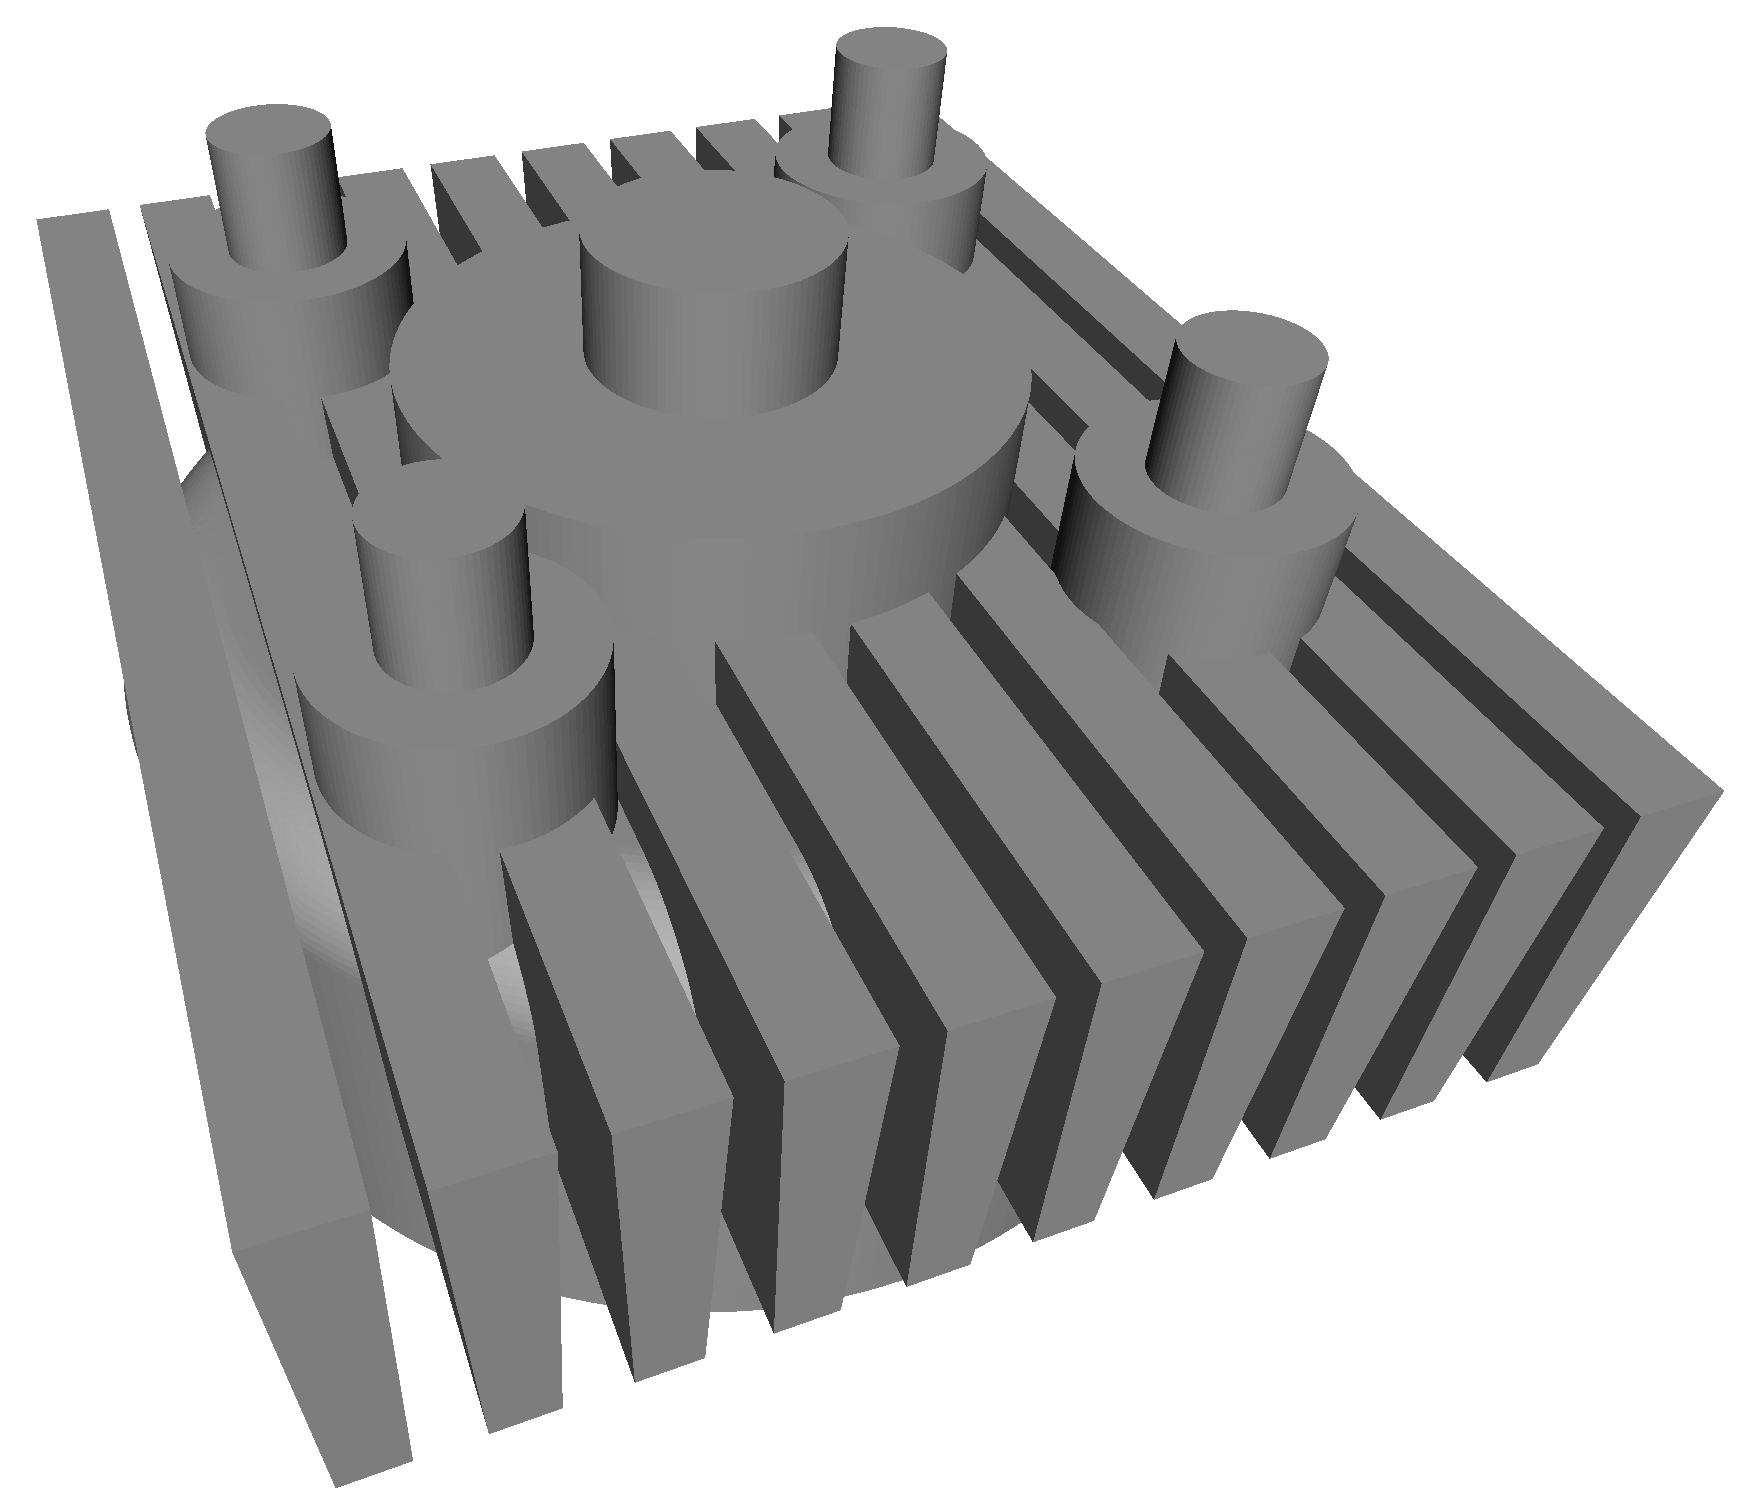
\includegraphics[width=\textwidth]{images/cylinder_head_stock_and_svs}
		\caption{Stock and SVs}
		\label{fig:cylinder_head_stock_sv}
	\end{subfigure}
	\begin{subfigure}[t]{0.32\textwidth}
		\centering
		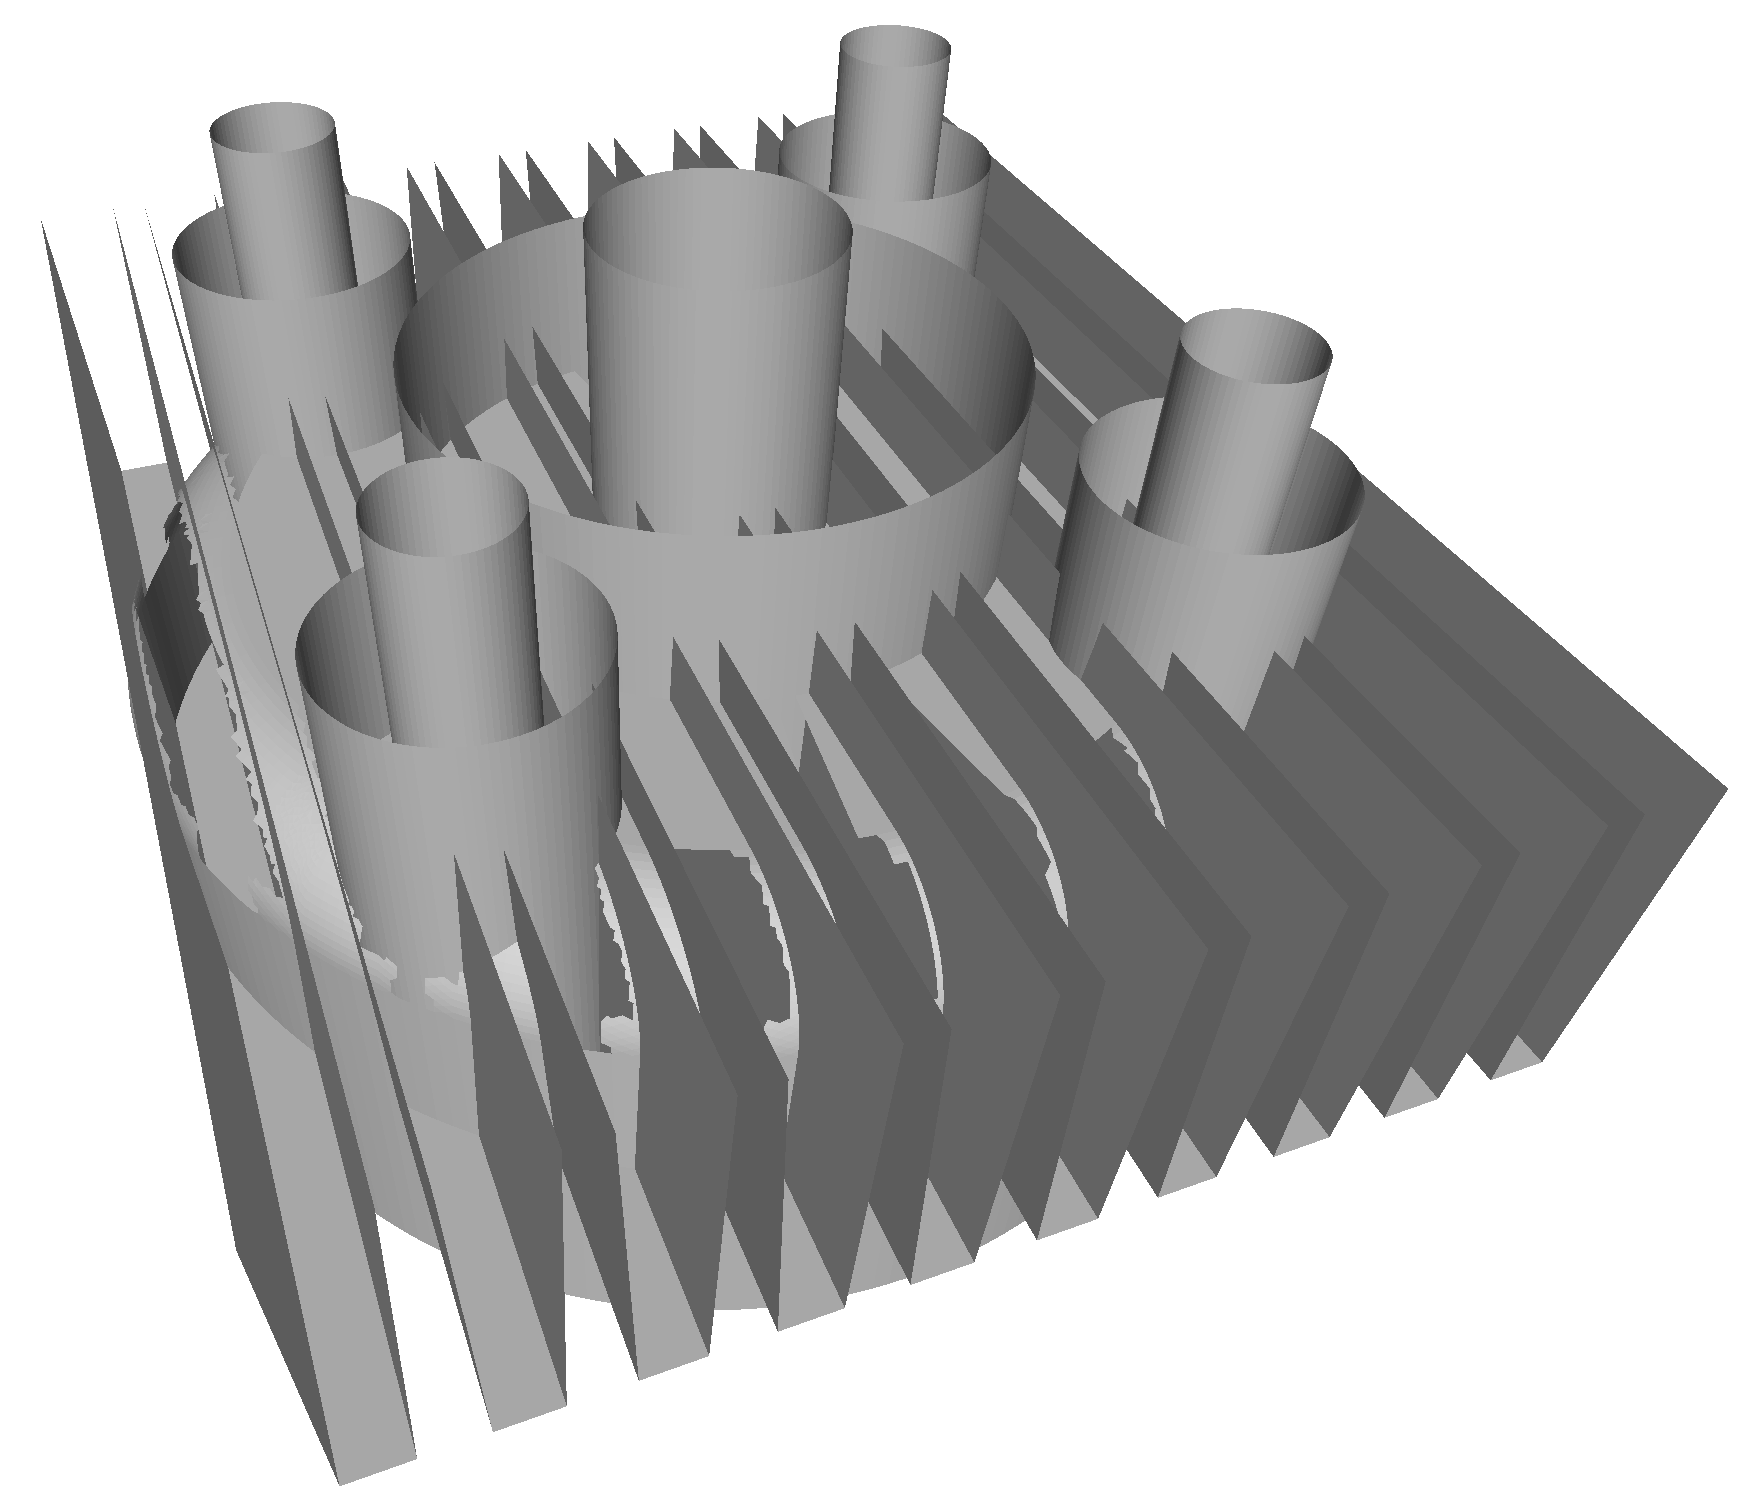
\includegraphics[width=\textwidth]{images/cylinder_head_vml}
		\caption{VML}
		\label{fig:cylinder_head_classified}
	\end{subfigure}
	\begin{subfigure}[t]{0.32\textwidth}
		\centering
		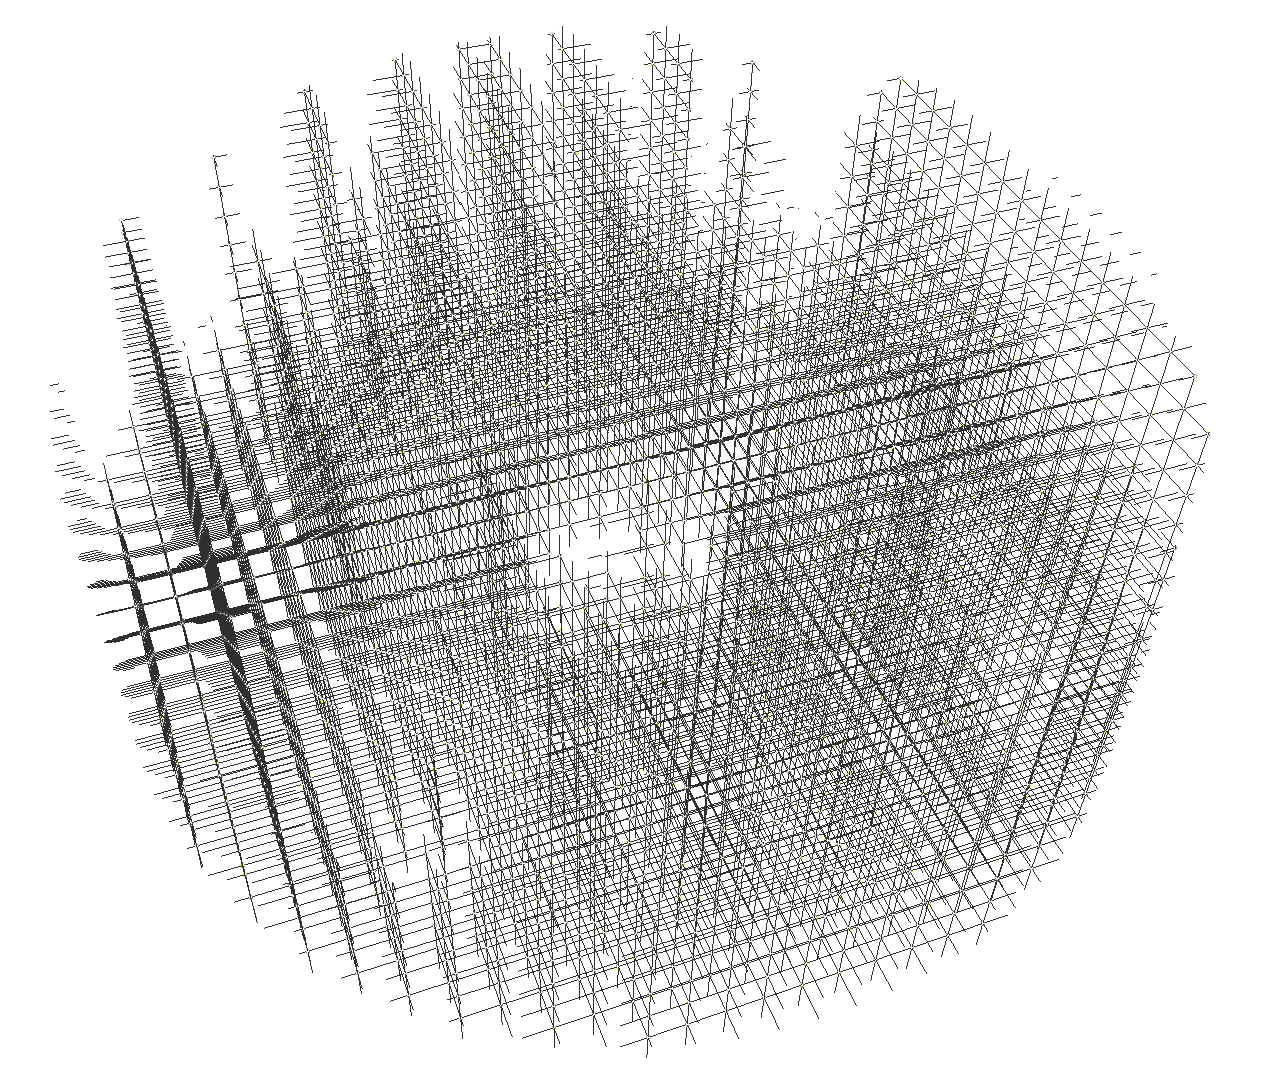
\includegraphics[width=\textwidth]{images/cylinder_head_dexel_image}
		\caption{Tri-dexel image}
		\label{fig:cylinder_head_dexel_image}
	\end{subfigure}
	\begin{subfigure}[t]{0.32\textwidth}
		\centering
		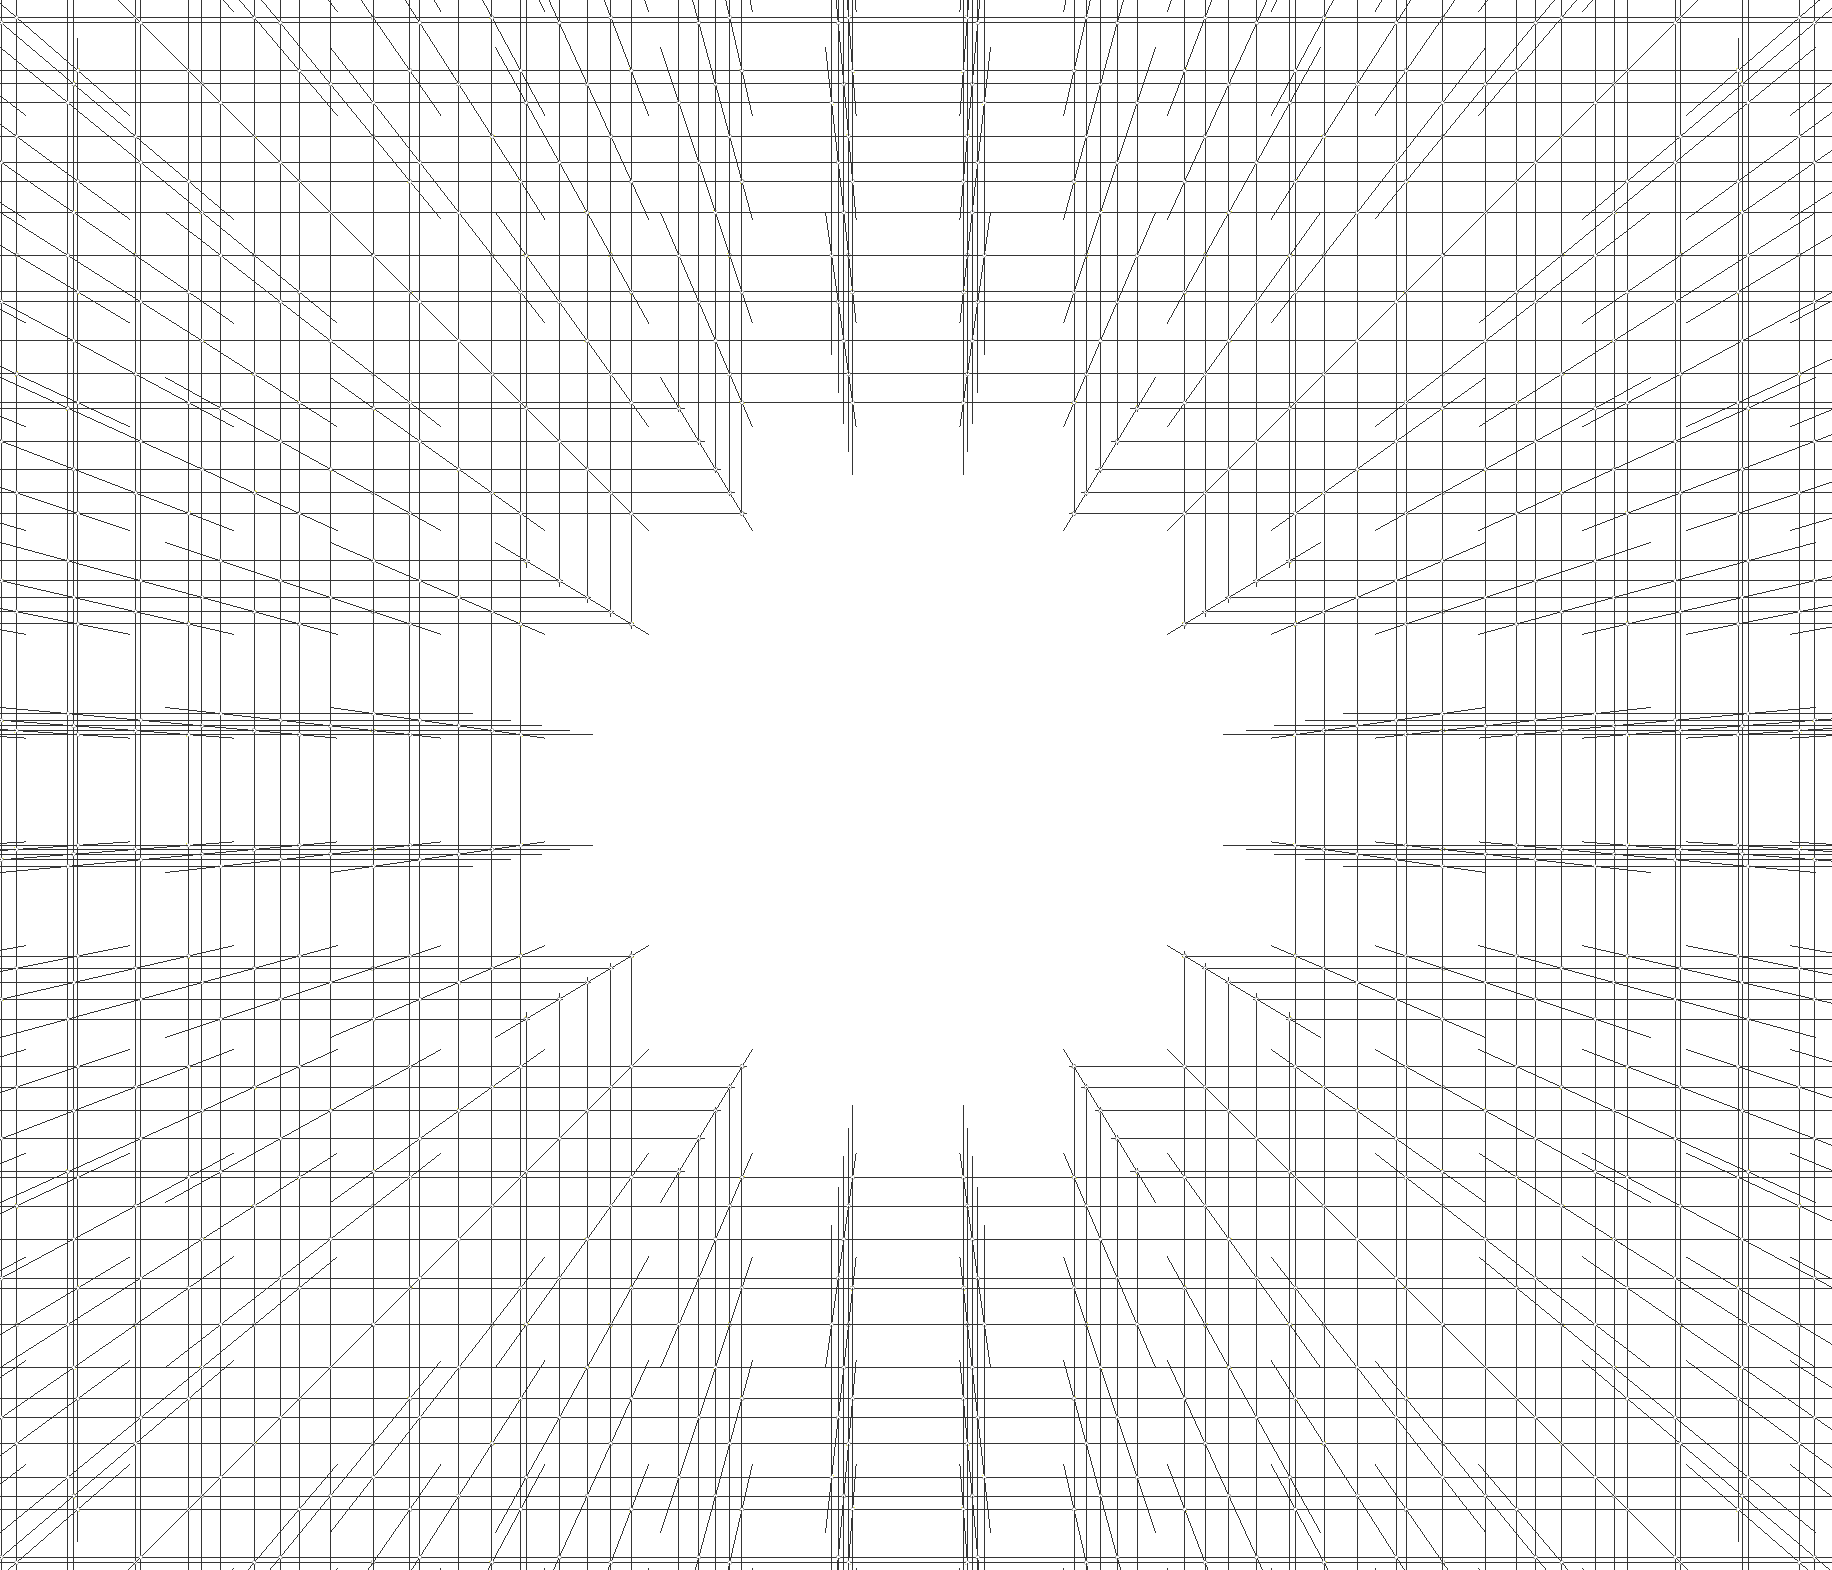
\includegraphics[width=\textwidth]{images/cylinder_head_dexel_image_center}
		\caption{Tri-dexel image center}
		\label{fig:cylinder_head_dexel_image_center}
	\end{subfigure}
	\begin{subfigure}[t]{0.32\textwidth}
		\centering
		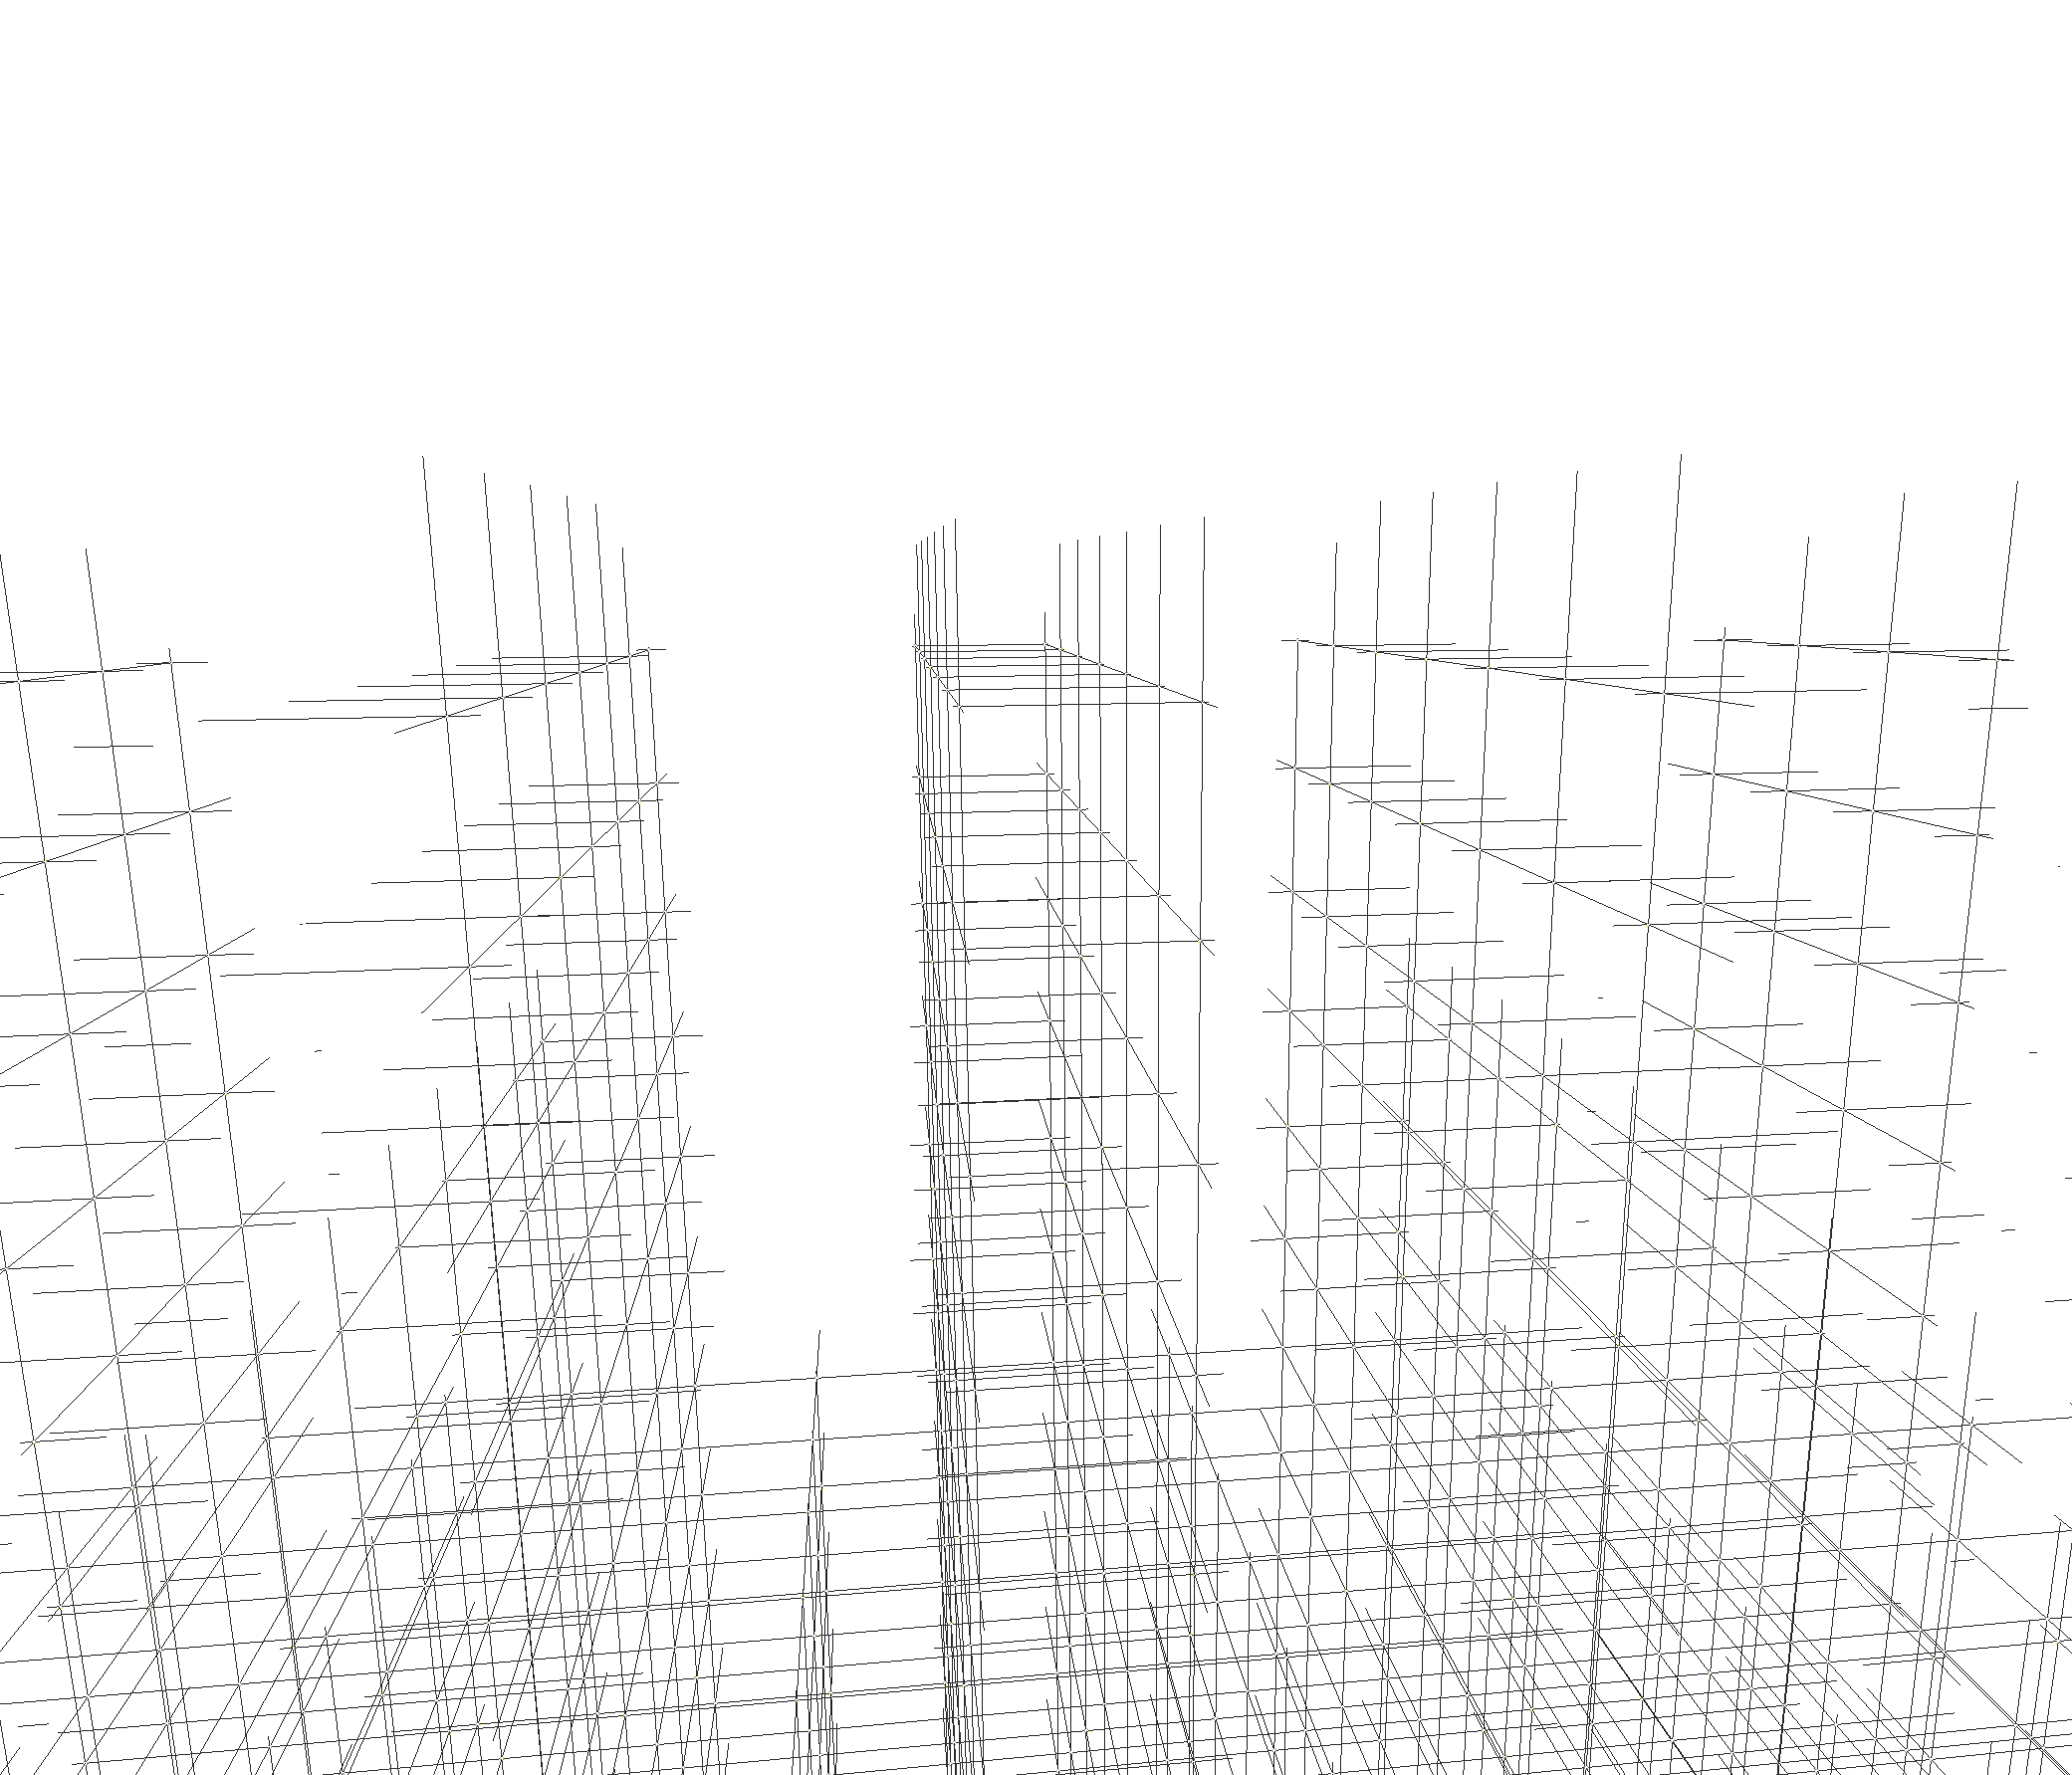
\includegraphics[width=\textwidth]{images/cylinder_head_dexel_image_fins}
		\caption{Tri-dexel image fins}
		\label{fig:cylinder_head_dexel_image_fins}
	\end{subfigure}
	\begin{subfigure}[t]{0.32\textwidth}
		\centering
		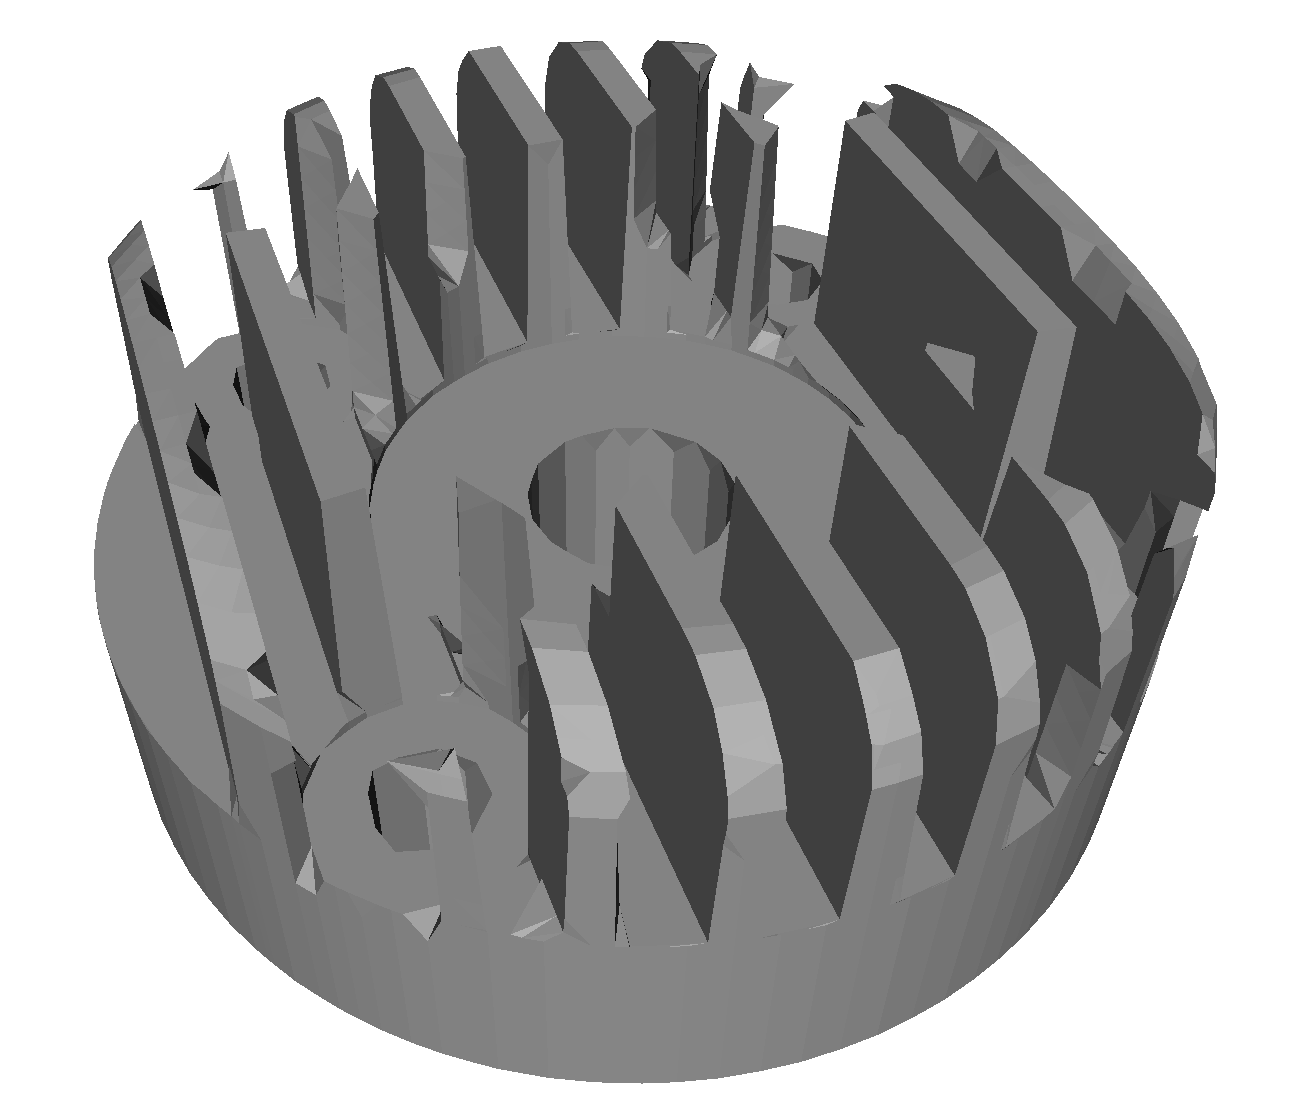
\includegraphics[width=\textwidth]{images/cylinder_head_reconstructed}
		\caption{Result}
		\label{fig:cylinder_head_reconstructed}
	\end{subfigure}
	\caption[Tri-dexel concept]{
		Tri-dexel based surface reconstruction from the data model of the VML of a cylinder head.
		The stock and a few swept volumes creating the fins and drillings are shown in \subref{fig:cylinder_head_stock_sv}.
		The classification result after these solids have been mapped into the regular grid of the VML is shown in \subref{fig:cylinder_head_classified}.
		The removed triangles are clearly visible, especially at the swept volumes.
		By using a raycast of axis-parallel rays along all three coordinate system axes a tri-dexel representation is created as shown in figure \subref{fig:cylinder_head_dexel_image}.
		The resolution of the grid spawning the rays is 30 along the longest dimension.
		Renderings of details of the tri-dexel image in \subref{fig:cylinder_head_dexel_image_center} and~\subref{fig:cylinder_head_dexel_image_fins} show the drilling at the center from above and the fins of the cylinder head from the center.
		Finally, the reconstructed surface is shown in \subref{fig:cylinder_head_reconstructed}.
		Note the imperfections at the edges and bases of the fins.
	}
	\label{fig:cylinder_head_dexel}
\end{figure}

In a subsequent step, the created tri-dexel representation is converted into a triangle mesh.
For this conversion, various algorithms are presented in literature.
A well-written algorithm by Ren \etal forms the idea and foundation of the implementation presented in this section \cite{tridexel_reconstruction}.
Triangulation is done independently for each grid cell.
Before a cell is triangulated, a few consistency checks and corrections are applied to the cell.
This process is called regularization and ensures a successful triangulation into a water-tight mesh.
For triangulation, a depth-first search process is iteratively started at non-occupied grid points of the cell to discover boundary loops.
Basically, the detected loops may be triangulated right away.
However, the quality of the triangulation is further enhanced by taking normal information at the dexel nodes into account.
This is especially necessary to reconstruct features of the model.
This optional feature reconstruction pass is run on the loops found in the previous step and may create additional vertices.
Taking these vertices into account allows the creation of better loop triangulations.


\subsection{Fundamentals}
\label{sec:tri_dexel_fundamentals}

Each intersection point of three orthogonal dexels from the tri-dexel grid forms a grid point.
If a grid point lies within a dexel segment on any of these dexels, it is said to be occupied.
The grid point thus lies within the volume of the workpiece.
Eight grid points and their twelve connecting edges along with their dexel segments are grouped into cells of the grid.
\Cref{fig:tri_dexel_cell} shows the structure of a tri-dexel cell.
%
\begin{figure}
	\centering
	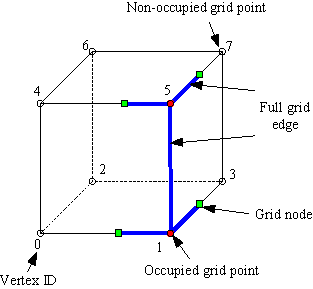
\includegraphics[width=0.5\textwidth]{images/tri_dexel_cell}
	\caption[Tri-dexel cell]{
		A cell of a tri-dexel grid, modified from \cite{tridexel_reconstruction}.
		Occupied grid points are drawn in red, dexel nodes in green, dexel segments in blue.
	}
	\label{fig:tri_dexel_cell}
\end{figure}
%
The edges of a tri-dexel cell contain dexel segments, or parts of them if the segment spans multiple cells.
At the end of each dexel segment is a dexel node, containing a depth value and a surface normal.
In the algorithms of this section, each grid point is referenced using a number between 0 and 7 and each edge using a number between 0 and 11.


\subsection{Overview}
\label{sec:tri_dexel_implementation}

In order to run the tri-dexel surface reconstruction, the user must supply a resolution as parameter.
This resolution determines the size of the raycasted dexel images as well as the resulting tri-dexel grid.
For esthetic reasons, the specified resolution is only used for the longest dimension of the workpiece.
The resolution along the other dimensions is usually smaller in order to make the cells more cubic, although the implementation does not require cubic cells.
This property will become important in an extension to the tri-dexel reconstruction discussed in \cref{sec:tri_dexel_cellslicing}.

In addition to the types already specified by the VML, \cf \cref{fig:vml_datamodel}, the tri-dexel reconstruction algorithm requires a few more types.
Most of these and also the algorithms themselves are vastly simplified when compared with the underlying source code.
Especially parallelism, asynchrony, memory efficient handling of data structures and numeric stability enhancements have been intentionally left out in the discussed pseudo code.


The additional types needed for the tri-dexel implementation are shown in the class diagram in \cref{fig:tri_dexel_datamodel}.
%
\begin{figure}
	\centering
	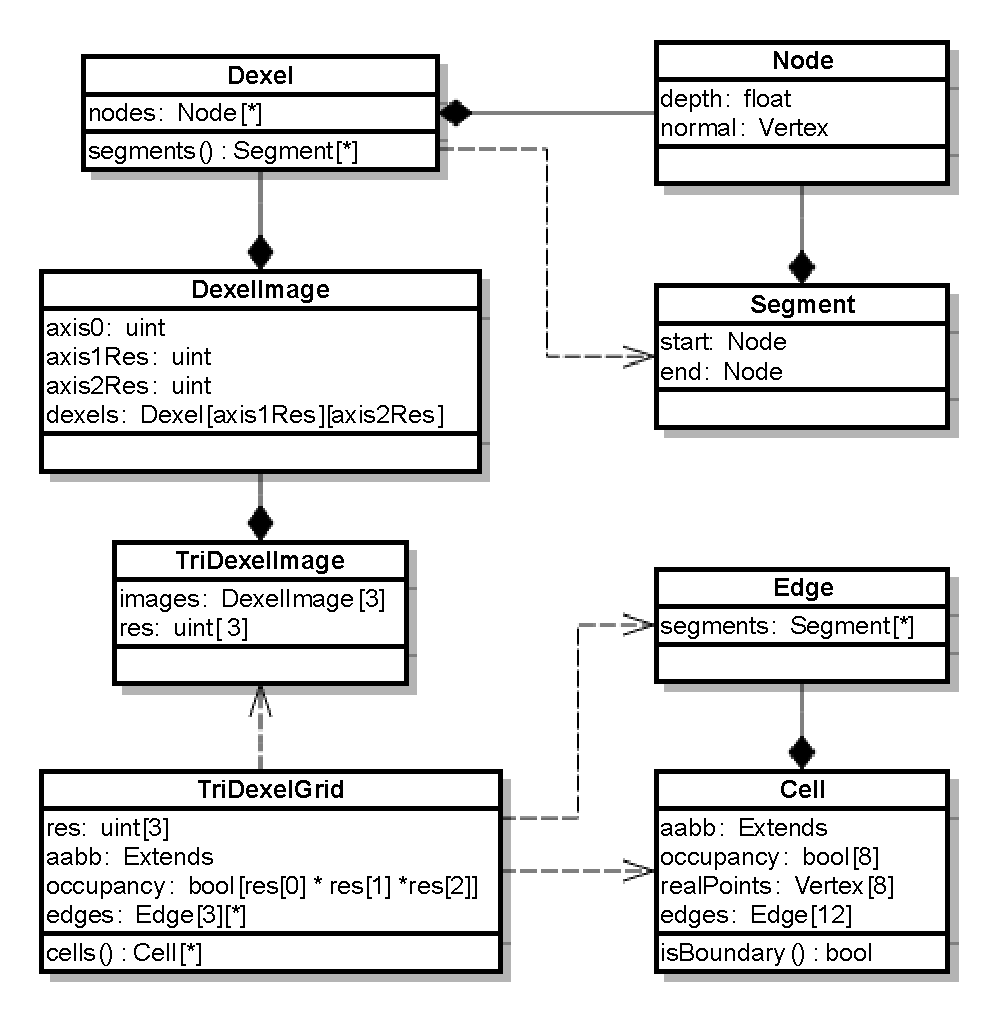
\includegraphics[width=0.9\textwidth]{images/tri_dexel_datamodel}
	\caption[Tri-dexel UML class diagram]{
		Simplified UML class diagram of the types needed for the tri-dexel reconstruction algorithm in addition to the types used by the VML, \cf \cref{fig:vml_datamodel}.
	}
	\label{fig:tri_dexel_datamodel}
\end{figure}
%
The most central data structure is the \var{TriDexelGrid} class.
It represents a tri-dexel representation of the complete VML workpiece, prepared for subsequent regularization and triangulation.
In addition to the resolution \var{res} and bounding box \var{aabb}, the \var{TriDexelGrid} class further contains the occupancy information for each grid point in \var{occupancy}, \ie whether a grid point is spanned by a dexel or not, as well as the actual dexel segments between the grid points, stored in \var{edges}.
The \var{cells} method separates all this information into distinct and independent cells.

Each cell is an instance of the \var{Cell} class and contains the same information as the tri-dexel grid, but locally for a single cell.
A cell stores its bounding box in \var{box}, the point occupancy of each of the corners corners in \var{occupancy}, the coordinates of the corners in \var{realPoints} and the twelve edges of the cell in \var{edges}.
Each edge of the cell is an instance of \var{Edge} and contains all spanning dexel segments, clamped to the interval between the incident grid points of the edge.
Furthermore, a method \var{isBoundary} is provided to check if the cell is a boundary cell, \ie contains occupied and non-occupied grid points, and therefore contains a part of the surface of the workpiece.

The \var{TriDexelGrid} is constructed from the \var{TriDexelImage} class, which, fundamentally, contains the same information as the tri-dexel grid.
The difference is substantially clearer from the perspective of the workflow.
Whereas the \var{TriDexelGrid} is already prepared for further processing, the \var{TriDexelImage} class only contains the raw data created by raycasting the data model of the VML.
This data only consists of the raycasting resolution \var{res} as well as three dexel images \var{images} along the three coordinate system axes.

A \var{DexelImage} describes the result of a single raycast along the axis specified in \var{axis0}, where 0 denotes the x-, 1 the y- and 2 the z-axis.
The members \var{axis1Res} and \var{axis2Res} store the resolution of the dexel image along the two cyclically following axes after \var{axis0}.
For example, if \var{axis0} is 1, the y-axis, then \var{axis1Res} and \var{axis2Res} hold the resolutions along the axes 2 and 0, the z- and x-axis.
Finally, \var{dexels} contains all the dexels of the image.

Each \var{Dexel} instance is then essentially a list of nodes, stored in \var{nodes}.
The number of stored nodes after raycasting is always a multiple of two.
As dexel nodes are typically processed in pairs, as dexel segments, a convenience method \var{segments} is provided, which groups adjacent nodes into instances of \var{DexelSegment}.

A \var{DexelSegment} contains these two nodes as \var{start} and \var{end} node.

Finally, the \var{Node} class holds the depth of the node along its dexel, \ie the distance of the node from the plane where the dexels originate, \cf \cref{fig:dexel_image}, as well as the normal vector of this surface entry/exit.

Unrelated to the tri-dexel types are two additional classes, which are used in some algorithms during the reconstruction.

The \var{Ray} class represents a ray starting at the vertex \var{origin} and traveling into the direction stored by \var{direction}.

The \var{EdgeVertex} class holds data to represent a vertex on an edge of a tri-dexel cell.
It contains grid point indices for the two points incident to the edge of this vertex, a position and the surface normal of the vertex.

Based on the discussed tri-dexel types, the basic reconstruction algorithm is shown in \cref{alg:tri_dexel}.
%
\begin{algorithm}
	\centering
	\begin{algorithmic}[1]
		\Function{TriDexel}{$\var{grid}, \var{resolution}$}
			\State $\var{box} = \var{Extends}(\var{grid}.\var{aabb}.\var{lower} - \epsilon_{\var{box}}, \var{grid}.\var{aabb}.\var{upper} + \epsilon_{\var{box}})$
			\State $\var{res} = \Call{UniformResolution}{\var{box}, \var{resolution}}$
			\State $\Call{Reconstruct}{\var{grid}, \var{box}, \var{resolution}}$
		\EndFunction
		\\
		\Function{Reconstruct}{$\var{grid}, \var{box}, \var{resolution}$}
			\State $\var{img} = \var{TriDexelImage}(\var{res})$ \label{line:tri_dexel_begin}
			\State $\Call{AxisParallelRaycast}{\var{grid}, \var{box}, \var{res},\hfill\break
				\hspace*{\dimexpr\algorithmicindent*2}(\var{axis}, \var{x}, \var{y}, \var{v}, \var{n}) \rightarrow \var{img}.\var{images}_{\var{axis}}.\var{dexels}_{\var{x}, \var{y}}.\var{nodes}.\var{add}(\var{Node}(\var{v}_{\var{axis}}, \var{n}))}$
			\State $\var{dgrid} = \Call{CreateTriDexelGrid}{\var{img}, \var{box}}$
			\State $\var{triangles} \gets \varnothing$
			\ForAll{$\var{cell} \in \var{dgrid}.\var{cells}()$}
				\State $\Call{RegularizeCell}{\var{cell}}$
				\State $\var{triangles} \gets \var{triangles} \cup \Call{TriangulateCell}{\var{cell}}$
			\EndFor
			\State \Return $\var{triangles}$
		\EndFunction
	\end{algorithmic}
	\caption[Tri-dexel workflow]{
		Abstract workflow of the surface reconstruction using a tri-dexel approach.
	}
	\label{alg:tri_dexel}
\end{algorithm}
%
At the beginning, a slightly enlarged bounding box is calculated for the size of the tri-dexel grid and raycast.
In this way, edge cases with a surface exactly at the border of the grid are avoided.
The \textproc{UniformResolution} function takes the user-specified resolution and the bounding box of the tri-dexel grid and calculates three resolutions, one for each axis.
The longest one is equal to the specified resolution and the other two are calculated in such a way that the resulting cells of the tri-dexel grid are as cubic as possible.
This tri-dexel grid resolution is used to preallocate space for the tri-dexel image, which is then filled in the subsequent raycasting process.
The remaining part of the algorithm closely follows the concept discussed in the previous \cref{sec:tri_dexel_concept}.
The subsequent sections discuss the functions and procedures of the algorithm in the order they are used.


\subsection{Raycast}
\label{sec:tri_dexel_raycast}

The raycast is the prime algorithm for converting the data model of the VML into a tri-dexel representation.
The raycast is performed with parallel, axis-aligned and equidistant rays.
All rays start at the intersection points of a uniform, 2-dimensional grid placed on one side of a slightly enlarged bounding box of the data model, and end at the opposite side, \cf \cref{fig:dexel_image}.
Three of these raycasts along the three axes of the coordinate system result in three dexel images.
As the raycasting code is kept separated from the tri-dexel data structures, a function is passed to the raycasting code which is invoked each time a ray has found a surface intersection.
Therefore, the same code is capable of creating other data structures as well, \cf \cref{sec:point_cloud_based}.

The entry routine and ray creation code of the raycasting algorithm is shown in \cref{alg:tri_dexel_raycast}.
%
\begin{algorithm}
	\centering
	\begin{algorithmic}[1]
		\Procedure{Raycast}{$\var{grid}, \var{box}, \var{res}, \var{hitFunc}$}
			\For{$\var{axis0} \gets 0 \To 2$}
				\State $\var{axis1} \gets (\var{axis0} + 1) \bmod 3$
				\State $\var{axis2} \gets (\var{axis0} + 2) \bmod 3$
				\State $\var{xCount} \gets \var{res}_{\var{axis1}}$
				\State $\var{yCount} \gets \var{res}_{\var{axis2}}$
				\State $\Delta \var{x} \gets (\var{box}.\var{upper}_{\var{axis1}} - \var{box}.\var{lower}_{\var{axis1}}) \div (\var{xCount} - 1)$
				\State $\Delta \var{y} \gets (\var{box}.\var{upper}_{\var{axis2}} - \var{box}.\var{lower}_{\var{axis2}}) \div (\var{yCount} - 1)$
				\For{$\var{y} \gets 0 \To \var{yCount} - 1$}
					\For{$\var{x} \gets 0 \To \var{xCount} - 1$}
						\State $\var{ray} = \Call{CreateRay}{\var{box}, \var{axis0}, \var{axis1}, \var{axis2}, \var{\Delta x}, \var{\Delta y}, \var{x}, \var{y}}$
						\State $\Call{CastRay}{\var{grid}, \var{axis0}, \var{axis1}, \var{axis2}, \var{ray},\hfill\break
							\hspace*{\dimexpr\algorithmicindent*5}(\var{v}, \var{n}) \rightarrow \var{hitFunc}(\var{axis0}, \var{x}, \var{y}, \var{v}, \var{n})}$
					\EndFor
				\EndFor
			\EndFor
		\EndProcedure
		\\
		\Function{CreateRay}{$\var{box}, \var{axis0}, \var{axis1}, \var{axis2}, \var{\Delta x}, \var{\Delta y}, \var{x}, \var{y}, \var{xCount}, \var{yCount}$}
			\State $\var{origin} \gets \var{box}.\var{lower}$
			\State $\var{origin}_{\var{axis1}} \gets \var{origin}_{\var{axis1}} + \var{x} \cdot \var{\Delta x}$
			\State $\var{origin}_{\var{axis2}} \gets \var{origin}_{\var{axis2}} + \var{y} \cdot \var{\Delta y}$
			\State $\var{direction} = \var{Vertex}(0, 0, 0)$
			\State $\var{direction}_{\var{axis0}} \gets 1$
			\State \Return $\var{Ray}(\var{origin}, \var{direction})$
		\EndFunction
		\\
		\Procedure{CastRay}{$\var{grid}, \var{axis0}, \var{axis1}, \var{axis2}, \var{ray}, \var{hitFunc}$}
			\State $\var{traverser} \gets \var{AxisAlignedTraverser}(\var{grid}, \var{ray}, \var{axis0}, \var{axis1}, \var{axis2})$
			\While{$\neg \var{traverser}.\var{reachedEnd}()$}
				\State $\var{cell} \gets \var{traverser}.\var{nextCell}()$
				\State $\Call{IntersectCell}{\var{cell}, \var{ray}, \var{axis0}, \var{axis1}, \var{axis2}, \var{hitFunc}}$
			\EndWhile
		\EndProcedure
	\end{algorithmic}
	\caption[Axis parallel raycast]{
		Basic algorithm for performing a parallel raycast along all three coordinate system axes on the data model of the VML.
	}
	\label{alg:tri_dexel_raycast}
\end{algorithm}
%
The outmost procedure \textproc{Raycast} takes four arguments: the regular grid data structure of the VML, the bounding box of the raycasted area, the resolution of the raycasted \enquote{image} as well as a function, which is called on every surface hit.
The algorithm starts off by iterating over the three axes of the coordinate system.
The index of each axis is stored in the variable \var{axis0}, where 0 denotes the x-, 1 the y- and 2 the z-axis.
\var{axis0} is also called primary axis and is accompanied by \var{axis1} and \var{axis2} which hold the other two, secondary axes, in cyclic order.
Depending on the choice of primary and secondary axes, the resolution of the 2-dimensional grid spawning the rays is determined and assigned to \var{xCount} and \var{yCount}, for the horizontal and vertical resolution.
The coordinate x and y inside the raycasting code refer to the axes of the raycasted \enquote{image} and not the axes of the 3-dimensional coordinate system of the scene.
Then, the distance between two incident rays along both secondary axes is computed.
Therefore, the size of the bounding box is computed and divided by the resolution minus one.
The result is assigned to the variables \var{\Delta x} and \var{\Delta y}.
Now, the algorithm starts creating and casting all rays along their primary axis.
Two nested loops iterate over all points of the 2-dimensional grid spawning rays.
For each grid point at $\var{x}, \var{y}$ a ray is created using the \textproc{CreateRay} function.
Subsequently, the ray is cast into the regular grid by invoking \textproc{CastRay}, passing a closure which is invoked each time a hit is recorded.

The objective of the \textproc{CreateRay} function is to create an instance of \var{Ray}, storing the origin and direction of the ray.
The origin is calculated by starting from the \var{lower} corner of the bounding box.
Along the primary axis, this value is already correct.
On the secondary axes, the origin, currently at the origin for ray $0, 0$, must be moved according to the \var{x} and \var{y} coordinate of the ray.
Thus, \var{x} and \var{y} are multiplied by the distances between incident rays, \var{\Delta x} and \var{\Delta y}, and added to the secondary axes of the origin.
%
Computing the direction of the ray is simpler, as it is axis aligned.
Therefore, the direction is a unit vector along the primary axis, created by setting the corresponding component of a zeroed vector to one.
%
Finally, \var{origin} and \var{direction} are aggregated into an instance of \var{Ray} and returned.

After rays have been created, they are cast into the regular grid of the VML using the \textproc{CastRay} procedure.
Traversing a ray through a regular grid is done using the 3D-DDA algorithm \cite{3DDDA}, \cf \cref{fig:traverser}.
However, as the rays are axis-parallel, traversal essentially boils down to mapping the origin of the ray to the appropriate grid cell and incrementing the 3-dimensional cell index along the primary axis until the other end of the grid is reached.
This logic is hidden behind the \var{AxisAlignedTraverser} class and is no further elaborated.

During traversal, the ray is intersected with each cell pulled from the traverser using the \textproc{IntersectCell} algorithm.
Fundamentally, the implementation is based on the inside counting scheme of the visualization code explained in \cref{fig:raycast}.
The important difference is that the raycast for visualization may terminate after the first intersection found.
Furthermore, minor inconsistencies are tolerable and may result in a few pixel errors on the final image.
However, when creating dexels, a consistent number of surface entries and exits as well as numerically correct ordering of the intersections is substantial.
Consequently, such an intersection routine must employ a great deal of numeric precautions and extra checks to deliver a correct result, even sacrificing intersections for the sake of consistency.
This procedure forms the heart of the raycasting algorithm.
As it is quite comprehensive and highly tailored to the internal data structures of the VML, the detailed pseudocode of the \textproc{IntersectCell} routine is omitted.


\subsection{Tri-dexel image and grid generation}
\label{sec:tri_dexel_dexel_image_generation}

Based on the generic, axis-parallel raycasting routine, a tri-dexel image is created in the base \cref{alg:tri_dexel}.
Before the raycast is launched, an instance of \var{TriDexelImage} is created, preallocating enough space to hold three dexel images, each holding a 2-dimensional grid of empty dexels.
When calling \textproc{AxisParallelRaycast}, an anonymous function is passed, which is invoked on every surface hit detected during raycasting.
This function receives the primary axis \var{axis}, \ie the axis along which the rays where traversed, \var{x} and \var{y} coordinate on the 2-dimensional dexel grid as well as the intersection point \var{v} with the normal of the hit triangle \var{n}.
With this information, the tri-dexel image stored in \var{img} is populated.
When raycasting is complete, the tri-dexel grid is generated from the tri-dexel image.
This conversion is more a reinterpretation and preparation of the information contained within the tri-dexel image.
Whereas the image contains the raw raycasting result, the tri-dexel grid already stores grid point occupancy information and cuts all dexels at cell borders.
This preparation eases the follow-up processing of individual cells.

Converting the tri-dexel image into a tri-dexel grid is achieved by the \textproc{CreateTriDexelGrid} function, which is shown in \cref{alg:tri_dexel_grid_generation}.
%
\begin{algorithm}
	\centering
	\begin{algorithmic}[1]
		\Function{CreateTriDexelGrid}{$\var{triImage}, \var{box}$}
			\State $\var{res} = \var{triImage}.\var{res}$
			\State $\var{grid} = \var{TriDexelGrid}(\var{res}, \var{box})$ \Comment{$\forall \var{x}, \var{y}, \var{z} \colon \var{grid}.\var{occupancy}_{\var{x}, \var{y}, \var{z}} = \False$}
			\For{$\var{axis0} \gets 0 \To 2$}
				\State $\var{axis1} \gets (\var{axis0} + 1) \bmod 3$
				\State $\var{axis2} \gets (\var{axis0} + 2) \bmod 3$
				\State $\var{image} \gets \var{triImage}.\var{images}_{\var{axis0}}$
				\For{$\var{axis1Val} \gets 0 \To \var{res}_{\var{axis1}} - 1$}
					\For{$\var{axis2Val} \gets 0 \To \var{res}_{\var{axis2}} - 1$}
						\State $\var{dexel} \gets \var{image}.\var{dexels}_{\var{axis1Val}, \var{axis2Val}}$
						\ForAll{$\var{seg} \in \var{dexel}.\var{segments}()$}
							\LineComment{Compute affected grid point range}
							\State $\var{start} \gets \Call{DepthToGrid}{\var{seg}.\var{start}.\var{depth}, \var{axis0}, \var{res}, \var{box}}$
							\State $\var{end} \gets \Call{DepthToGrid}{\var{seg}.\var{end}.\var{depth}, \var{axis0}, \var{res}, \var{box}}$
							\For{$\var{axis0Val} \gets \var{start} \To \var{end}$}
								%\State $\var{gridFrom} \gets (0, 0, 0)$
								\State $\var{gridFrom}_{\var{axis0}} \gets \var{axis0Val}$
								\State $\var{gridFrom}_{\var{axis1}} \gets \var{axis1Val}$
								\State $\var{gridFrom}_{\var{axis2}} \gets \var{axis2Val}$
								\State $\var{gridTo} \gets \var{gridFrom}$
								\State $\var{gridTo}_{\var{axis0}} \gets \var{gridTo}_{\var{axis0}} + 1$
								\State $\var{depthFrom} = \Call{GridToDepth}{\var{gridFrom}_{\var{axis0}}, \var{axis0}, \var{res}, \var{box}}$
								\State $\var{depthTo}   = \Call{GridToDepth}{\var{gridTo}_{\var{axis0}}, \var{axis0}, \var{res}, \var{box}}$
								\LineComment{Point occupancy}
								\If{$\var{seg}.\var{start}.\var{depth} \leq \var{depthFrom} \leq \var{seg}.\var{end}.\var{depth}$}
									\State $\var{grid}.\var{occupancy}_{\var{gridFrom}} \gets \True$
								\EndIf
								\If{$\var{seg}.\var{start}.\var{depth} \leq \var{depthTo} \leq \var{seg}.\var{end}.\var{depth}$}
									\State $\var{grid}.\var{occupancy}_{\var{gridTo}} \gets \True$
								\EndIf
								\LineComment{Copy segment and clamp to cell border}
								\State $\var{s} \gets \var{seg}$
								\If{$\var{s}.\var{start}.\var{depth} < \var{depthFrom}$}
									\State $\var{s}.\var{start}.\var{depth} \gets \var{depthFrom}$
								\EndIf
								\If{$\var{s}.\var{end}.\var{depth} > \var{depthTo}$}
									\State $\var{s}.\var{end}.\var{depth} \gets \var{depthTo}$
								\EndIf
								\State $\var{grid}.\var{edges}_{\var{axis0}, \var{gridFrom}}.\var{segments}.\var{add}(\var{s})$ \label{line:grid_edge_insertion}
							\EndFor
						\EndFor
					\EndFor
				\EndFor
			\EndFor
		\EndFunction
		\\
		\Function{DepthToGrid}{\var{depth}, \var{axis}, \var{res}, \var{box}}
			\State \Return $\floor{(\var{depth} - \var{box}.\var{lower}_{\var{axis}}) \div (\var{box}.\var{upper}_{\var{axis}} - \var{box}.\var{lower}_{\var{axis}}) \cdot (\var{res}_{\var{axis}} - 1)}$
		\EndFunction
		\\
		\Function{GridToDepth}{\var{gridCoord}, \var{axis}, \var{res}, \var{box}}
			\State \Return $\var{gridCoord} \div (\var{res}_{\var{axis}} - 1) \cdot (\var{box}.\var{upper}_{\var{axis}} - \var{box}.\var{lower}_{\var{axis}}) + \var{box}.\var{lower}_{\var{axis}}$
		\EndFunction
	\end{algorithmic}
	\caption[Tri-dexel grid creation]{
		Creating a tri-dexel grid from the raycasted dexel images.
	}
	\label{alg:tri_dexel_grid_generation}
\end{algorithm}
%
The algorithm starts by constructing an instance of the \var{TriDexelGrid} class.
During this construction, \ie the constructor, the occupancy of each grid point is set to \False.
Furthermore, space to hold all edges of the tri-dexel grid is allocated.
Accessing grid edges, \ie subscripting the member \var{edges}, is done by supplying the axis to which the edge is parallel as well as a three dimensional position.
Afterwards, the algorithm iterates over all three axes of the coordinate system and therefore over the three dexel images of the tri-dexel image.
For each dexel image further loops are necessary to iterate over all dexels of the image and for each dexel over its segments.

For each segment the affected range of grid points is computed.
Two coordinates of these points are already known, which are the same as the coordinates of the dexel in its image.
The third, missing coordinates are spanned by the dexel segment.
To compute these coordinates, the  start and end depth of the dexel segment are mapped to grid point coordinates.
Each call to \textproc{DepthToGrid} yields the lower grid point coordinate along the specified axis for a given depth on this axis.
This value is also equivalent to the index of the edge along \var{axis} on which a dexel node with the given depth would lie.
The computed range, \var{start} to \var{end}, in conjunction with \var{axis1Val} and \var{axis2Val}, now gives all indices of the affected grid points and edges.

The innermost loop finally iterates over all edges of the tri-dexel grid spanned by the current dexel segment \var{seg}.
The variables \var{gridFrom} and \var{gridTo} are the indices of the grid points incident to the current edge, which is also indexed by \var{gridFrom}.
For both grid points of the current edge a depth value along the current axis is calculated.
Two conditionals then compare these depth values against the start and end depth of the current dexel segment.
If the depth of any grid point is between the start and end depth of a dexel segment, \ie the segment spans the grid point, it is marked as occupied by setting the corresponding element of the \var{occupancy} member of the grid.
After this point occupancy check, the segment is added to the current edge, incident to the grid points \var{gridFrom} and \var{gridTo}.
As the cells of the tri-dexel grid are processed independently later and to ease calculations, the dexel-segments are further clamped to the bounds of a cell, \ie constrained to the range of the depth values of the cell of the grid point.
Therefore, a copy of the current segment is made and the start and end depth set to the respective depth values of the grid point, in case they are outside.
Finally, the clamped segment is added to the current edge.

After \textproc{CreateTriDexelGrid} returned, the tri-dexel image is no longer needed, as the semantically equivalent information is stored in the newly created tri-dexel grid.
The main algorithm, \cref{alg:tri_dexel}, may release resources held for the \var{img} variable now.

The newly created tri-dexel grid \var{dgrid} is now used to iterate over all cells and process them further.
The call to $\var{dgrid}.\var{cells}()$, for each cell, collects all data from the tri-dexel grid belonging to a single cell into an instance of \var{Cell}.
The created cells contain deep copies of the grid data, as the edges of the cell are shared with neighboring cells, but will be modified in subsequent parts of the algorithm.
This is no problem in a single threaded context, but would lead to data races when multiple cells are processed concurrently, \cf \cref{sec:tri_dexel_parallelization}.


\subsection{Regularization}
\label{sec:tri_dexel_regularization}

During the conversion of the data model of the VML into a tri-dexel representation errors may occur.
Dexel segments, for example, might not be of accurate length because of numeric instabilities in the triangle intersection routine or corrections applied by the raycaster when sorting and counting through the intersected structures to identify surface hits.
Such defects are especially critical at the intersection points of dexels from multiple dexel images, the grid points.
Furthermore, the number of different configurations a single tri-dexel cell may have is huge, as each edge may contain an arbitrary number of dexel segments, rendering the creation of an appropriate triangulation algorithm almost impossible.
Thus, it is beneficial to reduce the number of cases by dropping some information in favor of regularity.

The process of repairing defects and reducing complexity of a tri-dexel cell is called regularization.
This method is documented well in the tri-dexel work foundational to this chapter \cite{tridexel_reconstruction}.
Regularizing a tri-dexel cell is done by iterating over all edges and applying a set of rules.
These rules are illustrated in \cref{fig:tri_dexel_regularization} and described below:

\begin{figure}[h]
	%\renewcommand{\thesubfigure}{\arabic{subfigure}}
	\centering
	\begin{subfigure}[t]{0.45\textwidth}
		\centering
		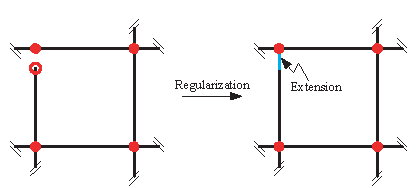
\includegraphics[width=\textwidth]{images/tri_dexel_regularization_1}
		\caption{Two occupied points.}
		\label{fig:tri_dexel_regularization_1}
	\end{subfigure}
	\begin{subfigure}[t]{0.45\textwidth}
		\centering
		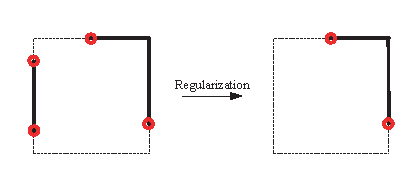
\includegraphics[width=\textwidth]{images/tri_dexel_regularization_2}
		\caption{Two non-occuupied points}
		\label{fig:tri_dexel_regularization_2}
	\end{subfigure}
	\begin{subfigure}[t]{0.45\textwidth}
		\centering
		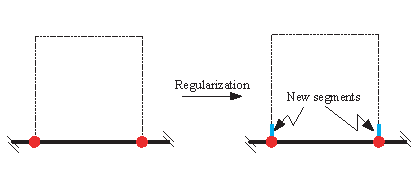
\includegraphics[width=\textwidth]{images/tri_dexel_regularization_3}
		\caption{One occupied point with no segment}
		\label{fig:tri_dexel_regularization_3}
	\end{subfigure}
	\begin{subfigure}[t]{0.45\textwidth}
		\centering
		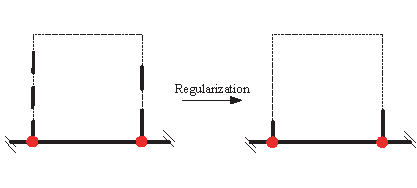
\includegraphics[width=\textwidth]{images/tri_dexel_regularization_4}
		\caption{Deletion of non-spanning segments}
		\label{fig:tri_dexel_regularization_4}
	\end{subfigure}
	\caption[Regularization rules]{
		The four regularization rules which are applied to each tri-dexel cell before it is triangulated.
		Image adapted from \cite{tridexel_reconstruction}.
	}
	\label{fig:tri_dexel_regularization}
\end{figure}

\begin{enumerate}
	\item If two adjacent grid points are marked as occupied, the incident edge must contain exactly one dexel segment with start and end depth exactly at the corresponding depths of the grid points.
	\Cref{fig:tri_dexel_regularization_1} shows the extension of the leftmost segment to touch the occupied grid point in the upper left.

	\item If two adjacent grid points are not marked as occupied, the incident edge must not contain any dexel segments.
	\Cref{fig:tri_dexel_regularization_2} shows the removal of the leftmost segment from an edge between two non-occupied grid points.

	\item If an edge, which is incident to only one occupied grid point, does not contain a dexel segment touching this point, a short segment is added, or, if a segment exists and is close enough to the occupied grid point, it is extended to touch the occupied point.
	\Cref{fig:tri_dexel_regularization_3} shows the creation of two small dexel segments at both lower grid points as the left and right edge do not contain any segments.

	\item If any segment does not touch any of the two incident grid points, it is removed.
	\Cref{fig:tri_dexel_regularization_4} shows the removal of segments on the left and right edge which do not touch any grid point.
\end{enumerate}

%These rules are applied to each cell of the tri-dexel grid constructed so far.
The implementation of these regularization rules, \ie the \textproc{RegularizeCell} routine, is detailed in \cref{alg:tri_dexel_regularization}.
%
\begin{algorithm}
	\centering
	\begin{algorithmic}[1]
		\Function{RegularizeCell}{$\var{cell}$}
			\For{$ \var{i} \gets 0 \To 11 $}
				\State $\var{segs} \gets \var{cell}.\var{edge}_{\var{i}}.\var{segments}$ \Comment{reference only}
				\label{line:reg_vars_begin}
				\State $(\var{src}, \var{dst}) \gets \var{edgeToPointIds}_{\var{i}}$
				\State $\var{axis} \gets \var{edgeToAxis}_{\var{src}, \var{dst}}$
				\State $\var{srcPoint} \gets \var{cell}.\var{realPoints}_{\var{src}}$
				\State $\var{dstPoint} \gets \var{cell}.\var{realPoints}_{\var{dst}}$
				\State $\var{srcDepth} \gets \var{srcPoint}_{\var{axis}}$
				\State $\var{dstDepth} \gets \var{dstPoint}_{\var{axis}}$
				\State $\var{srcOcc} \gets \var{cell}.\var{occupancy}_{\var{src}}$
				\State $\var{dstOcc} \gets \var{cell}.\var{occupancy}_{\var{dst}}$
				\label{line:reg_vars_end}

				\LineComment{Rule 1}
				\If{$\var{srcOcc} \wedge \var{dstOcc}$}
					\State $\var{n} \gets \var{Vertex}()$ \Comment{Invalid normal}
					\State $\var{segs} = \{ \var{Segment}(\var{Node}(\var{srcDepth}, \var{n}), \var{Node}(\var{dstDepth}, \var{n})) \}$
				\EndIf

				\LineComment{Rule 2}
				\If{$\neg \var{srcOcc} \wedge \neg \var{dstOcc}$}
					\State $\var{segs} \gets \varnothing$
				\EndIf

				\LineComment{Rule 3}
				\State $\var{n} = \var{Vertex}(0, 0, 0)$
				\State $\var{n}_{\var{axis}} = 1$
				\If{$\var{srcOcc} \wedge \neg \var{dstOcc}$}
					\If{$|\var{segs}| = 0 \vee \var{segs}_0.\var{start}.\var{depth} - \rho > \var{srcDepth}$}
						\State $\var{segs}.\var{add}(\var{Segment}(\var{Node}(\var{srcDepth}, -\var{n}), \var{Node}(\var{srcDepth} + \rho, \var{n})))$
					\ElsIf{$|\var{segs}| > 0 \wedge \var{segs}_0.\var{start}.\var{depth} > \var{srcDepth} \wedge {}$\hfill\break
						\hspace*{\dimexpr\algorithmicindent*4}$\var{segs}_0.\var{start}.\var{depth} - \rho \leq \var{srcDepth}$}
						\State $\var{segs}_0.\var{start}.\var{depth} \gets \var{srcDepth}$
					\EndIf
				\EndIf
				\If{$\neg \var{srcOcc} \wedge \var{dstOcc}$}
					\If{$|\var{segs}| = 0 \vee \var{segs}_{|\var{segs}| - 1}.\var{end}.\var{depth} + \rho < \var{dstDepth}$}
						\State $\var{segs}.\var{add}(\var{Segment}(\var{Node}(\var{dstDepth} - \rho, -\var{n}), \var{Node}(\var{dstDepth}, \var{n})))$
					\ElsIf{$|\var{segs}| > 0 \wedge \var{segs}_{|\var{segs}| - 1}.\var{end}.\var{depth} < \var{dstDepth} \wedge {}$\hfill\break
						\hspace*{\dimexpr\algorithmicindent*4}$\var{segs}_{|\var{segs}| - 1}.\var{end}.\var{depth} + \rho \geq \var{dstDepth}$}
						\State $\var{segs}_{|\var{segs}| - 1}.\var{end}.\var{depth} \gets \var{dstDepth}$
					\EndIf
				\EndIf

				\LineComment{Rule 4}
				\ForAll{$\var{s} \in \var{segs}$}
					\If{$\var{s}.\var{start}.\var{depth} \neq \var{srcDepth} \wedge \var{s}.\var{end}.\var{depth} \neq \var{dstDepth}$}
						\State $\var{segs}.\var{remove}(\var{s})$
					\EndIf
				\EndFor
			\EndFor
		\EndFunction
	\end{algorithmic}
	\caption[Regularizing]{
		Regularizing a cell of the tri-dexel grid by applying the four rules specified in \cref{fig:tri_dexel_regularization}.
	}
	\label{alg:tri_dexel_regularization}
\end{algorithm}
%
Regularizing a cell essentially boils down to processing all twelve edges of the cell, indexed from 0 to 11.
For each edge a bit of meta information is retrieved using some lookup tables.
These tables are shown in \cref{fig:tri_dexel_tables} and relate cell corners, edges and axes.
%
\begin{figure}
	\centering
	\begin{subfigure}[t]{0.25\textwidth}
		\centering
		\begin{align*}
			\intertext{neighborIds:}
			0 &\colon (1, 4, 2) \\
			1 &\colon (0, 3, 5) \\
			2 &\colon (0, 6, 3) \\
			3 &\colon (1, 2, 7) \\
			4 &\colon (0, 5, 6) \\
			5 &\colon (1, 7, 4) \\
			6 &\colon (2, 4, 7) \\
			7 &\colon (3, 6, 5)
		\end{align*}
	\end{subfigure}%
	\begin{subfigure}[t]{0.25\textwidth}
		\centering
		\begin{align*}
			\intertext{edgeToPointIds:}
			 0 &\colon (0, 1) \\
			 1 &\colon (2, 3) \\
			 2 &\colon (4, 5) \\
			 3 &\colon (6, 7) \\
			 4 &\colon (0, 2) \\
			 5 &\colon (1, 3) \\
			 6 &\colon (4, 6) \\
			 7 &\colon (5, 7) \\
			 8 &\colon (0, 4) \\
			 9 &\colon (1, 5) \\
			10 &\colon (2, 6) \\
			11 &\colon (3, 7)
		\end{align*}
	\end{subfigure}%
	\begin{subfigure}[t]{0.25\textwidth}
		\centering
		\begin{align*}
			\intertext{pointsToEdgeId:}
			(0, 1), (1, 0) &\colon  0 \\
			(2, 3), (3, 2) &\colon  1 \\
			(4, 5), (5, 4) &\colon  2 \\
			(6, 7), (7, 6) &\colon  3 \\
			(0, 2), (2, 0) &\colon  4 \\
			(1, 3), (3, 1) &\colon  5 \\
			(4, 6), (6, 4) &\colon  6 \\
			(5, 7), (7, 5) &\colon  7 \\
			(0, 4), (4, 0) &\colon  8 \\
			(1, 5), (5, 1) &\colon  9 \\
			(2, 6), (6, 2) &\colon 10 \\
			(3, 7), (7, 3) &\colon 11
		\end{align*}
	\end{subfigure}%
	\begin{subfigure}[t]{0.25\textwidth}
		\centering
		\begin{align*}
			\intertext{edgeToAxis:}
			(0, 1), (1, 0) &\colon 0 \\
			(2, 3), (3, 2) &\colon 0 \\
			(4, 5), (5, 4) &\colon 0 \\
			(6, 7), (7, 6) &\colon 0 \\
			(0, 2), (2, 0) &\colon 1 \\
			(1, 3), (3, 1) &\colon 1 \\
			(4, 6), (6, 4) &\colon 1 \\
			(5, 7), (7, 5) &\colon 1 \\
			(0, 4), (4, 0) &\colon 2 \\
			(1, 5), (5, 1) &\colon 2 \\
			(2, 6), (6, 2) &\colon 2 \\
			(3, 7), (7, 3) &\colon 2
		\end{align*}
	\end{subfigure}
	\begin{subfigure}[t]{0.4\textwidth}
		\centering
		\begin{align*}
			\intertext{cellSideNormals:}
			\binom{\{0, 2, 4, 6\}}{3} &\colon (         - 1,\phantom{-}0,\phantom{-}0) \\
			\binom{\{1, 3, 5, 7\}}{3} &\colon (\phantom{-}1,\phantom{-}0,\phantom{-}0) \\
			\binom{\{0, 1, 4, 5\}}{3} &\colon (\phantom{-}0,         - 1,\phantom{-}0) \\
			\binom{\{2, 3, 6, 7\}}{3} &\colon (\phantom{-}0,\phantom{-}1,\phantom{-}0) \\
			\binom{\{4, 5, 6, 7\}}{3} &\colon (\phantom{-}0,\phantom{-}0,         - 1) \\
			\binom{\{0, 1, 2, 3\}}{3} &\colon (\phantom{-}0,\phantom{-}0,\phantom{-}1) \\
		\end{align*}
	\end{subfigure}
	\caption[Helper tables]{
		Helper tables used by regularization and triangulation algorithms.
	}
	\label{fig:tri_dexel_tables}
\end{figure}
%
For a given edge index, the indices of the incident grid points are retrieved, called \var{src} and \var{dst}, where \var{src} is always the grid point with the lower depth value.
In addition to the index, the coordinate and occupancy is also retrieved in \var{srcPoint}, \var{dstPoint}, \var{srcOcc} and \var{dstOcc}.
Finally, the axis parallel to the edge is looked up and stored in \var{axis}.
Afterwards, the algorithm starts to apply the regularization rules.

For the first rule, the occupancy of both grid points is checked.
If both of them are occupied, the existing segments on the edge are replaced by a new set with a new segment spanning from the source to the destination grid point.
As both incident grid points are occupied, the edge cannot contain a surface intersection.
Therefore, the normals on the dexel nodes can be safely ignored.

The second rule states that if both grid points are not occupied, the incident edge must be empty.
Thus, in this case, all segments are simply replaced by an empty set.

Rule three is applied if only one grid point is marked as occupied.
If segments are present on the current edge, the algorithm tests whether the first or last segment touches the occupied grid point, or is very close to it.
If the source point is marked, the start of the first segment must touch or be near to it, \ie the depth of the start node  must not be further away from the grid point than a small $\rho$.
This length may be chosen arbitrarily, but as its purpose is to correct a numeric issue, a tiny value is sufficient.
In case the destination point is marked, the end of the last segment must touch or be near it.
If existing segments are nearer than $\rho$ to an occupied grid point, they are extended to reach it.
If there are no segments on the edge or the present segments are not in close proximity to their appropriate points, a new dexel segment is added.
The new segment starts at the occupied grid point and has a small length of $\rho$.
Regarding the normal, the surface intersection represented by the newly added segment might be used by a later triangulation.
However, the true normal is stored on the numerically too short segment in the appropriate neighboring cell, which is hard to retrieve as the cells of the tri-dexel grid are isolated to allow independent processing.
Hence, an artificial normal is added in the direction of axis parallel to the edge.

The last rule, rule four, finally checks all segments if they touch at least one grid point.
If any segment does not satisfy this condition, the segment is removed.

After all four rules have been applied to all twelve edges of the cell, the cell is regularized and fulfills a few properties:
\begin{itemize}
	\item Between two occupied grid points, there is always one full segment.
	\item Between two non-occupied grid points, there is never a segment.
	\item Between two differently marked grid points, there is exactly one segment with the depth of one node not equal to the depth of any grid point.
\end{itemize}
These properties now allow for a subsequent triangulation.


\subsection{Triangulation}
\label{sec:tri_dexel_triangulation}

After regularization, a cell of the tri-dexel grid is ready for triangulation.
The process of creating triangles from a cell is done in three steps where the second one is optional.
Firstly, set of boundary loops is created from the grid points and dexel nodes between them.
Secondly, from the loop, vertex and normal information, optional feature points are created.
Thirdly, the boundary loops with optional feature information are triangulated.

For the initial boundary loop detection, a depth-first search process is started at non-occupied grid points of the cell, one after the other.
The search traverses the edges of the cell and backtracks each time an occupied grid point and therefore a grid edge containing a dexel node is found.
Traversed grid points are marked as visited and cause future searches to backtrack immediately.
The list of visited grid edges containing dexel nodes, per search, in the order they were visited, form a boundary loop.
A cell might contain multiple boundary loops, which are found in multiple searches when starting at different, non-occupied grid points.

\Cref{fig:tri_dexel_triangulation} illustrates this depth-search process by two examples.
%
\begin{figure}
	\centering
	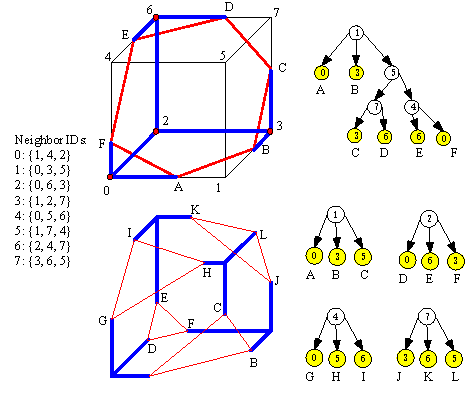
\includegraphics[width=0.9\textwidth]{images/tri_dexel_triangulation}
	\caption[Depth-first search loop discovery]{
		Triangulating a tri-dexel cell by finding boundary loops using depth-first search along the cube, starting at non-occupied nodes \cite{tridexel_reconstruction}.
	}
	\label{fig:tri_dexel_triangulation}
\end{figure}
%
In the upper example, a single boundary loop is discovered.
The search starts at grid point 1.
At each grid point, a list of neighbors has to be retrieved.
These neighbor ids make up a small table which is listed in \cref{fig:tri_dexel_tables} and beside the two examples in \cref{fig:tri_dexel_triangulation}.
The neighbors of a grid point are further traversed in counter-clockwise order, starting at the next neighbor after the one from which the current grid point has been reached.
At the first grid point of the search, the neighbor to start with may be chosen freely, and is usually the first one of the neighbor ids table.
At grid point 1, the neighbors 0, 3 and 5 are traversed.
Neighbors 0 and 3 reach an occupied grid point and therefore cause the search to backtrack, storing the dexel nodes A and B on the edges to 0 and 3.
As the neighbor 5 is non-occupied, the search continues with its neighbors, 1, 7, and 4.
Grid point 1 is omitted, as it has already been visited.
Grid point 7 is further traversed and backtracks at point 3 and 6, resulting in the dexel nodes C and D.
Grid point 4 produces the nodes E and F.
Finally, the search backtracks until the starting point is reached and terminates.
In visited order, the dexel nodes A to F form a boundary loop.
Further searches started at other grid points immediately return as all non-occupied nodes have already been visited by the search started at point 1.
%
In the lower example of \cref{fig:tri_dexel_triangulation}, the depth-first search discovers multiple boundary loops.

Triangulating a cell with occupancy information at its corners and vertices on its edges into triangles is a problem which is also discussed in voxel-based surface reconstruction techniques, such as the marching cubes variants.
In fact, a tri-dexel cell with eight Boolean occupancy values at the corners represents one of $2^8 = 256$ cases.
Therefore, the boundary loop configuration and also the triangulation could be precomputed for each case and stored in a lookup table.
This strategy is typically found in the original and many derived marching cubes implementations \cite{marching_cubes}.
As a matter of fact, the tables used by these marching cubes implementations, actually any table, could be used to triangulate tri-dexel cells.

Unfortunately, the depth-first search approach, as explained in the corresponding work \cite{tridexel_reconstruction}, does have an issue with four of the 256 configurations.
If only two grid points are occupied and lie on diagonally opposing corners of the cell, they form two boundary loops which are both discoverable by a single depth-first search.
This causes a problem, as the search discovers six vertices, which do not make up a single but two loops.
Therefore, these cases have to be handled differently.
A simple solution is to just start the depth-first search at the occupied grid points, resulting in two loops, and reverse the vertex order.

\Cref{alg:tri_dexel_triangulation} shows the basic triangulation of a tri-dexel cell without any feature reconstruction.
%
\begin{algorithm}
	\centering
	\begin{algorithmic}[1]
		\Function{TriangulateCell}{$\var{cell}$}
			%\State $loops$
			\If{$\neg \Call{IsProblematicCase}{\var{cell}}$}
				\State $\var{loops} \gets \Call{FindLoops}{\var{cell}, \False}$
			\Else
				\State $\var{loops} \gets \Call{ReverseLoops}{\Call{FindLoops}{\var{cell}, \True}}$
			\EndIf
			\State $\var{triangles} \gets \varnothing$
			\For{$\var{loop} \in \var{loops}$}
				\State $\var{triangles} \gets \var{triangles} \cup \Call{TriangulateLoopSimple}{\var{loop}}$
			\EndFor
			\State \Return $\var{triangles}$
		\EndFunction
		\\
		\Function{FindLoops}{$\var{cell}, \var{occupied}$}
			\State $\var{visited} \gets \var{array}(8, \False)$
			\State $\var{loops} \gets \varnothing$
			\For{$\var{start} \gets 0 \To 7$}
				\State $\var{loop} \gets \var{array}()$
				\State $\Call{DepthFirstSearch}{\var{occupied}, \var{start}, -1, \var{cell}, \var{visited}, \var{loop}}$
				\If{$|\var{loop}| > 0$}
					$\var{loops}.\var{add}(\var{loop})$
				\EndIf
			\EndFor
			\State \Return $\var{loops}$
		\EndFunction
		\\
		\Function{DepthFirstSearch}{$\var{occupied}, \var{cur}, \var{last}, \var{cell}, \var{visited}, \var{loop}$}
			\If{$\var{cell}.\var{occupancy}_{\var{cur}} = \var{occupied} \wedge \neg \var{visited}_{\var{cur}}$}
				\State $\var{visited}_{\var{cur}} \gets \True$
				\State $\var{neighbors} \gets \Call{RotateToStartAfter}{\var{neighborIds}_{\var{cur}}, \var{last}}$
				\For{$\var{n} \in \var{neighbors}$}
					\If{$\var{cell}.\var{occupancy}_{\var{n}} \neq \var{occupied}$}
						\State $\var{axis} \gets \var{edgeToAxis}_{\var{cur}, \var{n}}$
						\State $\var{seg} \gets \var{cell}.\var{edges}_{\var{pointsToEdgeId}_{\var{cur}, \var{n}}}.\var{segments}_0$
						\State $\var{curReal} \gets \var{cell}.\var{realPoints}_{\var{cur}}$
						\State $\var{nReal} \gets \var{cell}.\var{realPoints}_{\var{n}}$
						\If{$\var{seg}.\var{start}.\var{depth} = \var{curReal}_{\var{axis}} \vee \var{seg}.\var{start}.\var{depth} = \var{nReal}_{\var{axis}}$}
							\State $\var{node} \gets \var{seg}.\var{end}$
						\Else
							\State $\var{node} \gets \var{seg}.\var{start}$
						\EndIf
						\State $\var{v} \gets \var{curReal}$
						\State $\var{v}_{\var{axis}} \gets \var{node}.\var{depth}$
						\State $\var{loop}.\var{add}(\var{EdgeVertex}(\var{cur}, \var{n}, \var{v}, \var{node}.\var{normal}))$
					\Else
						\State $\Call{DepthFirstSearch}{\var{occupied}, \var{n}, \var{cur}, \var{cell}, \var{visited}, \var{loop}}$
					\EndIf
				\EndFor
			\EndIf
		\EndFunction
		\\
		\Function{TriangulateLoopSimple}{$\var{loop}$}
			\State $\var{vertices} \gets \Call{Map}{\var{loop}, \var{v} \rightarrow \var{v}.\var{position}}$
			\State \Return $\Call{TriangulateLoopIntoFan}{\var{vertices}}$
		\EndFunction
	\end{algorithmic}
	\caption[Depth-first search and basic triangulation]{
		Depth-first search and basic triangulating routine for a tri-dexel cell.
		No refinement or feature reconstruction is done.
	}
	\label{alg:tri_dexel_triangulation}
\end{algorithm}
%
The \textproc{TriangulateCell} function begins by checking if the cell is one of the four problematic cases, \ie cases with two, diagonally opposing occupied grid points.
In non-problematic cases, the \textproc{FindLoops} function is called, starting at non-occupied vertices.
In problematic cases, the loop search routine is started at occupied vertices and the resulting loops are reversed.

After all loops have been identified, they are sent to the \textproc{TriangulateLoopSimple} function which generates triangles from the loop.
The union of all triangulated loops is returned as triangulation result of the given tri-dexel cell.

The \textproc{FindLoops} algorithm is the entry into the depth-first search based traversal of the edges of the cell as shown in \cref{fig:tri_dexel_triangulation}.
It starts by initializing an array with eight Boolean values, set to false.
These values keep track of the already visited vertices.
For each of the eight possible start grid points an empty array \var{loop} is created, which is passed recursively through the following depth-first search.
It collects information about the encountered dexel nodes, in the order they are visited, to form a boundary loop.
The call to \textproc{DepthFirstSearch} then starts traversing the edges starting at the grid point \var{start}.
After the call has returned, a conditional checks if loop vertices have been found and adds the loop in this case.
After a search has been launched from each start point, the set of collected loops is returned.

The recursive \textproc{DepthFirstSearch} algorithm is the heart of the boundary loop discovery.
Initially, it checks if the current grid point is equal to \var{occupied} and has not been visited yet.
The parameter \var{occupied} is usually false for the default case, \ie the search traverses on non-occupied points, and only true in problematic cases.
If both conditions are met, the point is marked as visited and the list of neighbor points is fetched.
This list is rotated to start at the index right after the one the search came from.
This rotation ensures, that each neighbor is visited in counter-clockwise order as seen from the incoming edge.
In case of the first call to \textproc{DepthFirstSearch}, there is no last visited point, \var{last} is $-1$, and the neighbor list is not rotated.
On each neighboring grid point, its occupancy is checked for inequality to \var{occupied}.
If this is true, then \var{cur} and \var{n} have different occupancy and the edge between them contains a vertex of the surface.
This vertex is now constructed from the corresponding dexel node together with some meta data.
Using the \var{edgeToAxis} table of \cref{fig:tri_dexel_tables}, the axis parallel to the current edge is obtained.
Using \var{pointsToEdgeId}, the segment on the corresponding edge is also retrieved.
Furthermore, the coordinates of the current and neighboring grid point are stored in local variables.
The \var{node} variable is then set to the dexel node which does not touch one of the grid points.
The vertex on the current edge is then constructed starting with the coordinate of the current grid point \var{curReal}.
Choosing the coordinate of the neighboring grid point is also valid, as both coordinates only differ at the component at \var{axis}.
This component of the new vertex is then set to the depth of the selected node.
Finally, an instance of \var{EdgeVertex} is added to the boundary loop, containing the ids of both grid points, the newly calculated vertex and the corresponding surface normal as obtained from the dexel node.
As final step, the function returns and the search backtracks.
In case the occupancy of the current neighbor is equal to \var{occupied}, \ie no vertex on the current edge, the depth-first search is recursively continued with the current point index passed as last and the neighbor index passed as current.

Finally, in \cref{alg:tri_dexel_triangulation}, the \textproc{TriangulateLoopSimple} function just maps each \var{EdgeVertex} of the passed loop to its position, creating a pure list of 3-dimensional vertices.
These vertices are then sent to the \textproc{TriangulateLoopIntoFan} function, which creates a triangle fan from the given vertices around their center of mass.

The \textproc{TriangulateLoopIntoFan} function is one of three loop triangulation primitives used throughout this chapter.
These primitives are listed in \cref{alg:tri_dexel_loop_triangulation_primitives}.
%
\begin{algorithm}
	\centering
	\begin{algorithmic}[1]
		\Function{TriangulateLoopIntoFan}{$\var{loop}, \var{center}$}
			\If{$|\var{loop}| < 3$}
				\State \Return $\varnothing$
			\EndIf
			\State $\var{triangles} \gets \varnothing$
			\For{$\var{a} \gets 0 \To |\var{loop}| - 1$}
				\State $\var{b} \gets (\var{a} + 1) \mod |\var{loop}|$
				\State $\var{triangles}.\var{add}(\var{Triangle}(\var{center}, \var{loop}_{\var{a}}, \var{loop}_{\var{b}}))$
			\EndFor
			\State \Return $\var{triangles}$
		\EndFunction
		\\
		\Function{TriangulateLoopIntoFan}{$\var{loop}$}
			\State $\var{center} \gets \Call{Sum}{\var{loop}} \div |\var{loop}|$
			\State \Return $\Call{TriangulateLoopIntoFan}{\var{loop}, \var{center}}$
		\EndFunction
		\\
		\Function{TriangulateLoopAtFirst}{$\var{loop}, \var{center}$}
			\If{$|\var{loop}| < 3$}
				\State \Return $\varnothing$
			\EndIf
			\State $\var{center} \gets \var{loop}_0$
			\State $\var{triangles} \gets \varnothing$
			\For{$\var{b} \gets 2 \To |\var{loop}| - 1$}
				\State $\var{a} \gets (\var{b} - 1)$
				\State $\var{triangles}.\var{add}(\var{Triangle}(\var{center}, \var{loop}_{\var{a}}, \var{loop}_{\var{b}}))$
			\EndFor
			\State \Return $\var{triangles}$
		\EndFunction
	\end{algorithmic}
	\caption[Loop triangulation primitives]{
		Loop triangulation primitives.
	}
	\label{alg:tri_dexel_loop_triangulation_primitives}
\end{algorithm}
%
The \textproc{TriangulateLoopIntoFan} function is overloaded and, in its first version, takes two arguments, the loop to triangulate as well as the center of the triangulation.
The function initially checks if the loop contains at least three triangles and returns an empty set of triangles in this case.
Otherwise, a loop iterates over all adjacent pairs of vertices of the loop.
From each pair and the specified center, a triangle is instanced.
The set of all created triangles is returned at the end.

The single argument overload of \textproc{TriangulateLoopIntoFan} just takes a loop as argument and calculates the center itself as the centroid, \ie center of mass, of all loop vertices.
This is done by summing up all vertices and dividing the result by the number of vertices.

The \textproc{TriangulateLoopAtFirst} does also create a triangle fan.
However, this fan is centered on the first one of the loop vertices.
The code is similar to the \textproc{TriangulateLoopIntoFan} routine but spares a triangle at both index pairs containing the first vertex.
The resulting triangulation saves exactly two triangles in comparison with the \textproc{TriangulateLoopIntoFan} approach.


\subsection{Refinement and feature reconstruction}
\label{sec:tri_dexel_refinement}

The triangulation shown in the last \cref{sec:tri_dexel_triangulation}, \textproc{TriangulateLoopSimple} in \cref{alg:tri_dexel_triangulation}, is very basic and does not use the per-vertex normal information.
However, this additional data is helpful and allows to refine the generated surface and reconstruct features like sharp edges and corners.
In order to do so, the \textproc{TriangulateLoopSimple} routine is replaced by a more comprehensive algorithm, which makes use of the vertex normals to calculate additional feature vertices before triangulation.
Two types of feature information is calculated:
Using the normals of each pair of adjacent vertices of the loop, an additional intermediate vertex may be created.
Using the normals of multiple vertices, a further apex vertex may be created, one per loop.
Finally, these enhanced loops are also triangulated.

\Cref{fig:tri_dexel_refinement} sketches both cases.
The drawing on the left shows the creation of two intermediate vertices.
The one on the right shows the creation of three intermediate vertices and the calculation of an apex vertex.
%
\begin{figure}
	\centering
	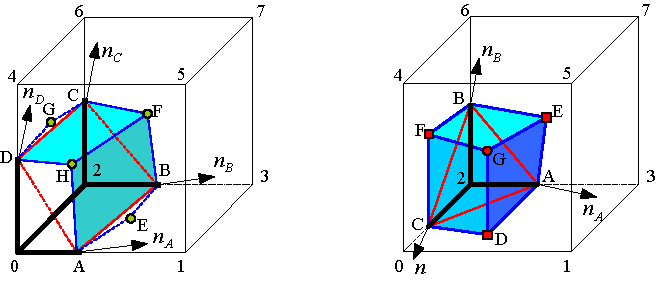
\includegraphics[width=0.9\textwidth]{images/tri_dexel_refinement}
	\caption[Feature reconstruction]{
		Triangulating the boundary loops of a tri-dexel cell with additional feature information \cite{tridexel_reconstruction}.
		The left image shows the creation of two intermediate vertices, F and H.
		The right image shows the creation of three intermediate vertices, D, E and F, and an apex vertex, G.
	}
	\label{fig:tri_dexel_refinement}
\end{figure}
%
All feature points are calculated using the intersection of three planes.
For the intermediate vertices between two adjacent loop vertices, two planes are given by the normals of the two vertices and one plane is given by the cell side containing both vertices.

On the left of \cref{fig:tri_dexel_refinement}, the original boundary loop consists of the vertices A, B, C, and D.
Each of these points holds an additional normal, $n_A$, $n_B$, $n_C$ and $n_D$.
Now, the intermediate point G for example is calculated from the two planes described by the positions and normals of D and C and the cell side to the left.
Using this scheme, an intermediate vertex is calculated for each adjacent pair of vertices on the boundary loop.
In case the calculated vertex is too close to the original edge or lies outside the bounding box of the cell, the vertex is discarded.
The vertices G and E are too close to their edges CD and AB and discarded, whereas vertex H and F are kept.

If at least three intermediate vertices are created, an additional apex vertex may be calculated, again as intersection of three planes.
For these planes, the first three loop vertices are taken, which have resulted in the construction of a valid intermediate vertex.
In the right drawing of \cref{fig:tri_dexel_refinement}, the loop vertices A, B and C have resulted in intermediate vertices, namely D, E and F.
The first three of them, A, B, and C, are then used to form three planes which intersect in the apex point G.
The location of the apex is also checked against the bounding box of the cell.
In case it is outside, the apex is discarded again.

Finally, after creating intermediate and apex vertices, the enhanced boundary loops must be triangulated.
This task is not as easy as the simple triangulation of a loop, as some cases must be distinguish, depending on the availability of intermediate and apex vertices.
%In case a valid apex vertex has been created, the intermediate vertices are placed between the original loop vertices and the resulting loop is triangulated into a fan with the apex vertex as center.
%Otherwise, if no intermediate vertex is found at all, the initial loop is just triangulated into a fan with its center of mass as center, \cf \textproc{TriangulateLoopSimple}.
%If one intermediate vertex is found, the loop is triangulated with the intermediate vertex as center.
%If more than one intermediate vertex is found, the loop is split into subloops.
%Each sequence of an intermediate vertex, an arbitrary number of original loop vertices and another intermediate vertex is triangulated.
%This loop clipping is repeated until only one loop with intermediate vertices is left, which is also triangulated.

\Cref{alg:tri_dexel_refinement} describes the details of the refinement and feature reconstruction pass, creating enhanced boundary loops for triangulation.
This algorithm acts as a replacement for the \textproc{TriangulateLoopSimple} function of \cref{alg:tri_dexel_triangulation}.
%
\begin{algorithm}
	\centering
	\begin{algorithmic}[1]
		\Function{TriangulateLoopRefined}{$\var{loop}, \var{cell}$}
			\State $\var{inside} \gets \var{p} \rightarrow \var{cell}.\var{aabb}.\var{lower} < \var{p} < \var{cell}.\var{aabb}.\var{upper}$
			\State $\var{apexVertices} \gets \var{array}()$
			\State $\var{finalLoop} \gets \var{array}()$
			\State $\var{isEdgeVertex} \gets \var{array}()$
			\State $\var{intermedCount} = 0$
			\LineComment{Create new boundary loop with intermediate vertices}
			\For{$\var{i} \gets 0 \To |\var{loop}| - 1$}
				\State $\var{a} \gets \var{loop}_{\var{i}}$
				\State $\var{b} \gets \var{loop}_{(\var{i} + 1) \mod |\var{loop}|}$
				\State $\var{finalLoop}.\var{add}(\var{a}.\var{position})$
				\State $\var{isEdgeVertex}.\var{add}(\True)$
				\State $\var{points} \gets \Call{Unique}{(\var{a}.\var{point}, \var{a}.\var{neigbor}, \var{b}.\var{point}, \var{b}.\var{neighbor})}$
				\State $\var{n} \gets \var{cellSideNormals}_{\var{points}_0, \var{points}_1, \var{points}_2}$
				\State $\var{cellPlane} \gets \var{Plane}(\var{n}, \var{cell}.\var{realPoints}_{\var{points}_0})$
				\State $\var{aPlane} \gets \var{Plane}(\var{a}.\var{normal}, \var{a}.\var{position})$
				\State $\var{bPlane} \gets \var{Plane}(\var{b}.\var{normal}, \var{b}.\var{position})$
				\State $\var{intermed} \gets \Call{IntersectPlanes}{\var{cellPlane}, \var{aPlane}, \var{bPlane}}$
				\If{$\var{intermed} \wedge \var{inside}(\var{intermediate})$}
					\State $\var{dist} \gets \Call{PointLineDistance}{\var{a}.\var{position}, \var{b}.\var{position}, \var{intermed}}$
					\If{$\var{dist} > \epsilon_{\var{line}}$}
						\State $\var{finalLoop}.\var{add}(\var{intermed})$
						\State $\var{isEdgeVertex}.\var{add}(\False)$
						\State $\var{intermedCount} \gets \var{intermedCount} + 1$
						\State $\var{apexVertices}.\var{add}(\var{a})$
						\State $\var{apexVertices}.\var{add}(\var{b})$
					\EndIf
				\EndIf
			\EndFor
			\LineComment{Try to create an apex vertex}
			\If{$\var{intermedCount} \geq 3$}
				\State $\var{apexVertices} \gets \Call{Unique}{\var{apexVertices}}$
				\State $\var{planes} \gets \var{array}()$
				\For{$\var{i} \gets 0 \To 2$}
					\State $\var{planes}.\var{add}(\var{Plane}(\var{apexVertices}_{\var{i}}.\var{normal}, \var{apexVertices}_{\var{i}}.\var{position}))$
				\EndFor
				\State $\var{a} \gets \Call{IntersectPlanes}{\var{planes}_0, \var{planes}_1, \var{planes}_2}$
				\If{$\var{a} \wedge \var{inside}(\var{a})$}
					\State $\var{apex} \gets \var{a}$
				\EndIf
			\EndIf
			\State $\dots$
		\algstore{refinement}
	\end{algorithmic}
	\caption[Feature reconstruction 1]{
		Feature reconstruction by calculating intermediate vertices and an optiona apex based on the original boundary loops.
		The algorithm is continued in \cref{alg:tri_dexel_refinement_triangulation}.
	}
	\label{alg:tri_dexel_refinement}
\end{algorithm}
%
In the beginning, a closure is created to test if a point is inside the bounding box of the passed cell.
Then, a few arrays are created.
One contains a list of vertices which have led to a valid intermediate point and may be considered for creating an apex vertex, called \var{apexVertices}.
The variable \var{finalLoop} will contain the original vertices of the boundary loop interleaved with the created intermediate vertices.
The \var{isEdgeVertex} array complements the \var{finalLoop} array, as it stores a Boolean value for each of the vertices in the final loop.
This Boolean value is true if the vertex at the same index originated from an edge of the cell and false if the vertex is an intermediate vertex.
Finally, a counter for the number of successfully created intermediate vertices is created and initialized to zero.
A loop iterates over all vertices \var{a} and their successors \var{b}, \ie adjacent pairs, of vertices of the original loop.
Vertex \var{a} is added to the final loop and \True to \var{isEdgeVertex}.
The four grid point indices of both edge vertices are collected and uniqued.
As both edge vertices share a common side of the cell, the result is a list of grid point indices with either three or four elements, depending on whether or not one of them is shared.
Three of these indices uniquely identify one of the sides of the cell and are used as indices into another lookup table, \var{cellSideNormals}, storing the normal of a cell side for each combination of three grid points.
The normal is retrieved using the first three grid points of the current edge vertex pair and stored in \var{n}.
Now, three planes are created, one using the normal of the cell side and the coordinate of a grid point on this cell side and two others from the pair of edge vertices.
By calling \textproc{IntersectPlanes}, the intersection point of the three planes is calculated, which is a possible intermediate vertex.
The returned result in \var{intermed} is tested for validity as \textproc{IntersectPlanes} may return an empty result if no intersection could be found.
Furthermore, the intersection point must lie within the bounds of the cell.
If these conditions are satisfied, the distance from the line between the pair of vertices to the calculated intersection point is measured.
If this distance is larger than a specified and small $\epsilon_{\var{line}}$, the intersection point is accepted as an intermediate vertex.
It is therefore added to the final loop.
As it is not an edge vertex, \False is added to the \var{isEdgeVertex} list.
Furthermore, the intermediate vertex counter is incremented and both edge vertices are added to the list of candidates for apex creation.

After all edge vertex pairs of the initial loop have been processed and all intermediate vertices have been created, an apex vertex may be generated.
Therefore, the number of emitted intermediate vertices is checked.
If this number is larger than or equal to three, the first three unique edge vertices are used to create three planes which are again intersected.
In case an intersection point could be found and it also lies within the bounding box of the cell, it is accepted as valid apex vertex.

Now, enough information has been gathered from the normal information at each vertex to begin triangulating the loop.
This second part of the \textproc{TriangulateLoopRefined} function is listed in \cref{alg:tri_dexel_refinement_triangulation}.
%
\begin{algorithm}
	\centering
	\begin{algorithmic}[1]
		\algrestore{refinement}
			\State $\dots$
			\If{$\var{apex}$}
				\State \Return $\Call{TriangulateLoopIntoFan}{\var{finalLoop}, \var{apex}}$
			\ElsIf{$\var{intermedCount} = 0$}
				\State \Return $\Call{TriangulateLoopIntoFan}{\var{finalLoop}}$
			\ElsIf{$\var{intermedCount} = 1$}
				\State $\Call{Rotate}{\var{finalLoop}, \Call{FindFirst}{\var{isEdgeVertex}, \False}}$
				\State \Return $\Call{TriangulateLoopAtFirst}{\var{finalLoop}}$
			\Else
				\State $\var{triangles} \gets \varnothing$
				\For{$\var{first} \gets 0 \To |\var{finalLoop}| - 1$} \Comment{Reevaluated at each iteration}
					\If{$\neg \var{isEdgeVertex}_{\var{first}}$}
						\State $\var{last} \gets (\var{first} + 1) \mod |\var{finalLoop}|$
						\While{$\var{isEdgeVertex}_{\var{last}}$}
							\State $\var{last} \gets (\var{last} + 1) \mod |\var{finalLoop}|$
						\EndWhile
						\State $\var{subLoop} \gets \var{array}()$
						\For{$\var{i} \gets (\var{first} \To \var{last}) \mod |\var{finalLoop}|$}
							\State $\var{subLoop}.\var{add}(\var{finalLoop}_{\var{i}})$
						\EndFor
						\State $\var{triangles} \gets \var{triangles} \cup \Call{TriangulateLoopIntoFan}{\var{subLoop}}$
						\State $\Call{RemoveCyclicRange}{\var{finalLoop}, \var{first} + 1, \var{last} - 1}$
						\State $\Call{RemoveCyclicRange}{\var{isEdgeVertex}, \var{first} + 1, \var{last} - 1}$
					\EndIf
				\EndFor
				\State $\var{triangles} \gets \var{triangles} \cup \Call{TriangulateLoopIntoFan}{\var{finalLoop}}$
				\State \Return $\var{triangles}$
			\EndIf
		\EndFunction
		\\
		\Function{IntersectPlanes}{$\var{a}, \var{b}, \var{c}$}
			\State $\var{det} \gets \begin{vmatrix} \var{a}.\var{normal} & \var{b}.\var{normal} & \var{c}.\var{normal} \end{vmatrix}$
			\If{$|\var{det}| > \epsilon_{\var{plane}}$}
				\State \Return $((\var{b}.\var{normal} \times \var{c}.\var{normal}) \cdot \var{a}.\var{dist} + {}$\hfill\break
				\hspace*{\dimexpr\algorithmicindent*2}\phantom{\Return $($}$(\var{c}.\var{normal} \times \var{a}.\var{normal}) \cdot \var{b}.\var{dist} + {}$\hfill\break
				\hspace*{\dimexpr\algorithmicindent*2}\phantom{\Return $($}$(\var{a}.\var{normal} \times \var{b}.\var{normal}) \cdot \var{c}.\var{dist}) \div \var{det}$
			\EndIf
			\LineComment{Otherwise, return nothing}
		\EndFunction
		\\
		\Function{PointLineDistance}{$\var{a}, \var{b}, \var{p}$}
			\State \Return $|(\var{p} - \var{a}) \times (\var{p} - \var{b})| \div |\var{a} - \var{b}|$
		\EndFunction
	\end{algorithmic}
	\caption[Feature reconstruction 2]{
		Continuation of \cref{alg:tri_dexel_refinement}.
		Triangulation of a boundary loop enhanced with intermediate vertices and an optional apex.
	}
	\label{alg:tri_dexel_refinement_triangulation}
\end{algorithm}
%
For the triangulation of the loop, enriched with intermediate vertices and an optional apex vertex, several cases have to be distinguished, depending on the available data.

If an apex vertex has been found, the final loop containing edge and intermediate vertices is directly triangulated into a fan with the apex vertex as center.

If no apex and intermediate vertices have been found, the loop is triangulated the same way as in the \textproc{TriangulateLoopSimple} version, by creating a fan around the loops centroid.

If no apex and one intermediate vertex are found, the loop is triangulated as a fan around the intermediate vertex.
Therefore, the loop is rotated to start with the intermediate vertex and then passed to \textproc{TriangulateLoopAtFirst}.

Loops with no apex vertex and more than one intermediate vertex are more difficult to triangulate.
The case illustrated in \cref{fig:tri_dexel_refinement} on the left shows that the final loop must actually split into two sub loops, one containing C, D, H and F, as well as one containing A, B, D, H.
This fact becomes even clearer with cases like the one on the right if the apex vertex was invalid, \eg the apex G would be outside the bounding box of the cell.
In this case, all intermediate vertices D, E and F would form a plateau.
The remaining parts of the final loop are sub loops, each consisting of two neighboring intermediate vertices and the edge vertices in-between.

This sub loop clipping strategy is now algorithmically applied to \var{finalLoop}.
A for loop iterates over the indices of all vertices, each the first element of a potential sub loop.
If the vertex at this current index is not an edge vertex, \ie an intermediate vertex, then a nested loop searches the next, cyclically occurring intermediate vertex on the loop, skipping all edge vertices in between.
After it has been found, the inclusive range from \var{first} to \var{last} contains a sub loop, which is now copied from \var{finalLoop} and triangulated into a fan.
Afterwards, the edge vertices of the sub loop are removed from \var{finalLoop} and \var{isEdgeVertex}.
After all such sub loops have been clipped and triangulated, \var{finalLoop} consists only of intermediate vertices.
These are also triangulated.
The union of the triangulations of all sub loops and the remaining final loop forms the triangulation of the complete boundary loop and is returned.

Throughout the \textproc{TriangulateLoopRefined} function, two helper functions are used.
The first, \textproc{IntersectPlanes}, calculates the intersection point between three planes.
A good algorithm for this problem is found in the Graphics Gems series \cite[p304]{graphics_gems_1}.
It describes the intersection point as the solution of a system of linear equations as follows:
For three planes with normals $n_a$, $n_b$, $n_c$, stored as column vectors, and distances $d_a$, $d_b$, $d_c$, intersecting at $x$, $y$, $z$, using the variables
\begin{equation}
	N = \begin{bmatrix} n_a, n_b, n_c \end{bmatrix}, \;
	I = \begin{bmatrix} x \\ y \\ z \end{bmatrix}, \;
	d = \begin{bmatrix} d_a \\ d_b \\ d_c \end{bmatrix},
\end{equation}
the system
\begin{equation}
N I = d
\end{equation}
is solved using Cramer's rule
\begin{equation}
	x = \frac{\begin{vmatrix} d, n_b, n_c \end{vmatrix}}{|N|}, \;
	y = \frac{\begin{vmatrix} n_a, d, n_c \end{vmatrix}}{|N|}, \;
	z = \frac{\begin{vmatrix} n_a, n_b, d \end{vmatrix}}{|N|} \text{.}
\end{equation}
By describing the intersection point as
\begin{equation}
	I =
	x \begin{bmatrix} 1 \\ 0 \\ 0 \end{bmatrix} +
	y \begin{bmatrix} 0 \\ 1 \\ 0 \end{bmatrix} +
	z \begin{bmatrix} 0 \\ 0 \\ 1 \end{bmatrix} \text{,}
\end{equation}
substituting $x$, $y$ and $z$ and expanding the determinant into a triple product, the equation becomes
\begin{equation}
	I =
	\frac{d \times n_b \cdot n_c}{|N|} \begin{bmatrix} 1 \\ 0 \\ 0 \end{bmatrix} +
	\frac{n_a \times d \cdot n_c}{|N|} \begin{bmatrix} 0 \\ 1 \\ 0 \end{bmatrix} +
	\frac{n_a \times n_b \cdot d}{|N|} \begin{bmatrix} 0 \\ 0 \\ 1 \end{bmatrix} \text{.}
\end{equation}
As the operands of the triple product can be rotated, $d$ is isolated from the cross product.
Then, the vectors after the fractions are lifted onto the numerator and multiplied with $d$, extracting the components $d_a$, $d_b$ and $d_c$, resulting in
\begin{equation}
I =
	\frac{n_b \times n_c \cdot d_a}{|N|} +
	\frac{n_c \times n_a \cdot d_b}{|N|} +
	\frac{n_a \times n_b \cdot d_c}{|N|} \text{.}
\end{equation}
By combining all three fractions, the equation for the intersection calculation, which is used by the \textproc{IntersectPlanes} function, is complete.
If the determinant of matrix $N$ becomes zero, two of the contained normal vectors and therefore planes are parallel.
Determinants close to zero, \ie smaller than $\epsilon_{\var{plane}}$, may further cause numeric issues when calculating the intersection point.
Therefore, in this case, the function does not return a result, \ie a result which always evaluates to \False in Boolean expressions.

The function \textproc{PointLineDistance} computes the closest distance of a point \var{p} to the line defined by two other points \var{a} and \var{b}.
The implemented variant to solve this problem \cite{point_line_distance}, computes the length of the cross product between the two vectors from \var{p} to both line endings.
This value is the doubled area of the triangle \var{a}, \var{b}, \var{c}, where the line distance is the altitude of the triangle.
Dividing the doubled area by the base of the triangle, \ie the length of the line $\overline{\var{a}\var{b}}$, the point to line distance is obtained.


\subsection{Cell slicing}
\label{sec:tri_dexel_cellslicing}

With the additional refinement and feature reconstruction introduced in \cref{sec:tri_dexel_refinement}, the quality of the tri-dexel surface reconstruction is improved appreciably.
Still, features within a cell and especially thin features not crossing any grid points are almost fully discarded.
The reason therefore is the the destructive regularization step described in \cref{sec:tri_dexel_regularization}, which sacrifices smaller dexel segments in favor of regularity, throwing away useful information, especially of smaller features.
To preserve this information and still obtain regular tri-dexel cells, which can be passed into the triangulation routines of \cref{sec:tri_dexel_triangulation,sec:tri_dexel_refinement}, an alternative to the regularization algorithm has been developed.
This novel approach depends on the ability to resample dexels at any time, an ability usually not given in scenarios where the dexel model is the main data model, \ie typical, dexel-based machining simulations.
However, as the dexel model used for surface reconstruction is derived from the internal data model of the VML, it allows to arbitrarily recreate dexels.

\begin{figure}
	\centering
	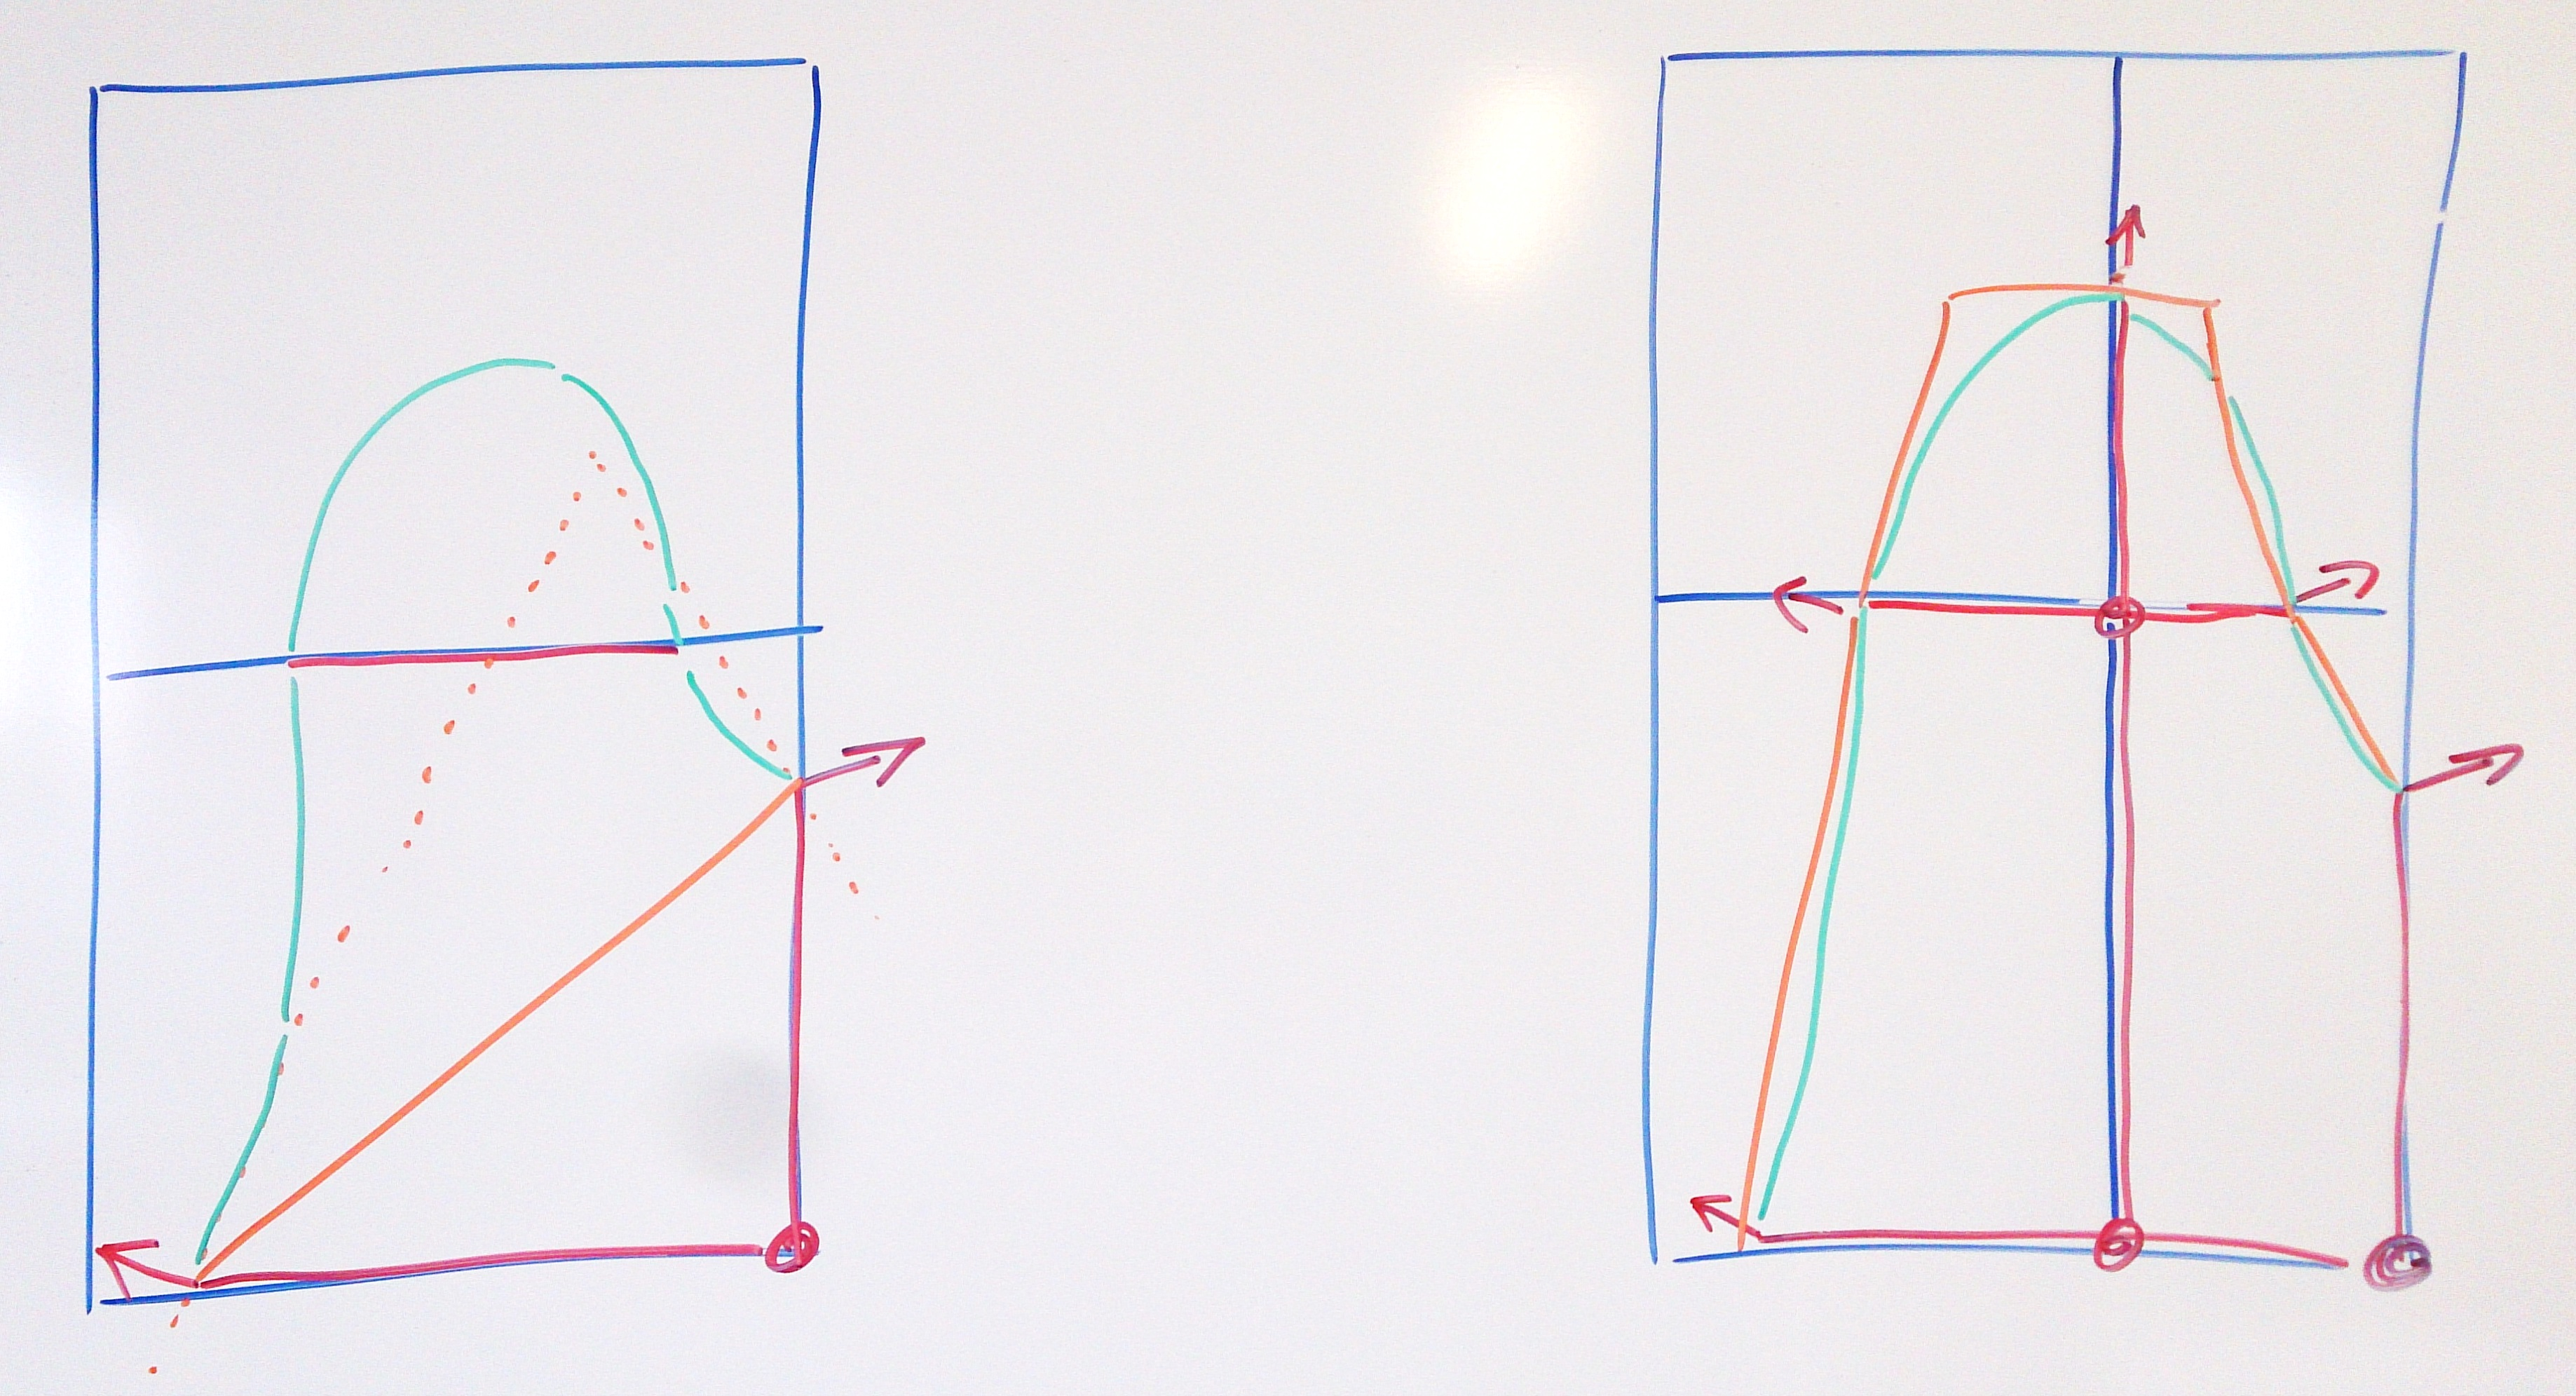
\includegraphics[width=0.7\textwidth]{images/tri_dexel_cellslicing}
	\caption[Cell slicing]{
		Creating regular cells by slicing two irregular cells sharing an irregular edge.
		The actual surface is drawn in green, the reconstructed one in red.
		A possible intermediate vertex in the left scenario is discarded, as it is outside the bounding box of the cell.
	}
	\label{fig:tri_dexel_cellslicing}
\end{figure}

The main problem of small dexel segments is that they are always lost during regularization if they do not pass a grid point of the tri-dexel grid.
If a lot of fine features are shed this way, an obvious solution is to increase the resolution of the dexel grid.
However, this solution dramatically increases memory and computational demands and also adds detail where it is not necessary, \eg in large flat surfaces or empty space.
A smarter solution is to increase the grid resolution locally.
More specifically, each irregular cell, \ie a cell which contains irregular edges which have to be modified by the regularization, is subdivided in such a way that all irregular edges become regular, without modifying the segments.
This subdivision is accomplished by calculating divider planes for each irregular cell.
As much planes as necessary are created to slice all segments or empty spaces between segments, which would be discarded by the regularization.
\Cref{fig:tri_dexel_cellslicing} shows this procedure by an example.
The left drawing shows a small feature which will be lost due to regularization as the edge shared by both cells is irregular; regularization rule two will remove the segment.
As the calculated intermediate point lies outside the lower cell, \cf dotted lines in red, the quality of the reconstructed surface is poor.
The right image shows the same situation with an additional divider line (plane in 3D).
The divider is resampled, creating new dexel segments.
All resulting four cells are now regular and, after triangulation, produce a good surface approximation.

Nevertheless, after slicing irregular cells to ensure regularity on the edges, the resampled dexels within the cell might again produce irregular cells.
Therefore, this cell slicing technique is applied recursively.
As the detail of the reconstructed surface is increased on each subdivision at the cost of more and finer triangles, the use of a maximum recursion depth is advised.
When this limit is hit, the cell, despite being irregular, is passed to the standard regularization algorithm, discarding the now hopefully expendable features.

\begin{figure}
	\centering
	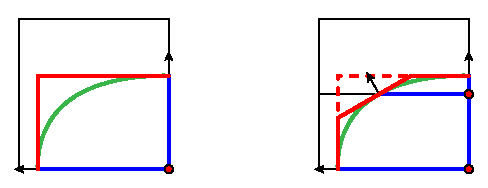
\includegraphics[width=0.9\textwidth]{images/tri_dexel_hole_creation}
	\caption[Cell slicing creating a hole]{
		Creating a hole at the border of a normal and a sliced cell by estimating different feature points.
		The original surface is drawn in green, the reconstructed one in red.
	}
	\label{fig:tri_dexel_hole_creation}
\end{figure}

Adaptively slicing cells and resampling the model to a higher level of detail in distinct places is dangerous and may create thin holes on the surface.
The tri-dexel reconstruction algorithm usually generates a closed manifold by assuming that the same feature points and edges are created by two adjacent cells at their common border.
If one of the cells is sliced, feature points might be estimated differently.
\Cref{fig:tri_dexel_hole_creation} shows an example of a case where a hole is created between a normal and a sliced cell.
The sketch on the left shows a cell side estimating a feature point based on the dexel segments at the edges of the cell.
The sketch on the right shows the side of the adjacent cell, which has been sliced, \eg by another irregular edge at the opposite cell side.
Due to the additional information gathered by the resampled dexel at the slicing plane, two feature points are calculated in the sliced cell, instead of one in the unsliced cell.
Thus, a different surface is created at the border, resulting in a typically thin hole.

The cells resulting from slicing are resampled, regularized and triangulated by reusing all existing classes and algorithms.
For each cell a new tri-dexel image is created with a resolution of two in each dimension with exactly the same bounding box as the cell.
The reconstruction procedure is similar to algorithm forming the main tri-dexel image, \cf \cref{alg:tri_dexel} \cref{line:tri_dexel_begin}ff.

This new cell slicing algorithm is integrated into the existing code by adapting the base tri-dexel reconstruction algorithm, \cref{alg:tri_dexel}, as shown in \cref{alg:tri_dexel_2}.
%
\begin{algorithm}
	\centering
	\begin{algorithmic}[1]
		\setalglineno{6}
		\Function{Reconstruct}{$grid, box, resolution$}\hfill\break
			\hspace*{\dimexpr\algorithmicindent*1}\dots
			\setalglineno{11}
			\ForAll{$\var{cell} \in \var{dgrid}.\var{cells}()$}
				\If{$\Call{RegularizeCell}{\var{cell}, \True}$}
					\State $\var{triangles} \gets \var{triangles} \cup \Call{TriangulateCell}{\var{cell}}$
				\Else
					\State $\var{triangles} \gets \var{triangles} \cup \Call{SliceCell}{\var{cell}, \var{grid}}$
				\EndIf
			\EndFor
			\State \Return $\var{triangles}$
		\EndFunction
	\end{algorithmic}
	\caption[Cell slicing workflow]{
		Adaption to the abstract workflow given in \cref{alg:tri_dexel} to support cell slicing.
	}
	\label{alg:tri_dexel_2}
\end{algorithm}
%
The \textproc{RegularizeCell} procedure is slightly adapted.
A Boolean value is added to its interface and, if cell slicing is allowed, a value \True is passed to \textproc{RegularizeCell}, indicating that only numeric regularizations, \cf regularization rule three, are allowed and other necessary regularizations, \ie irregular edges, are only detected but not applied.
A Boolean return value of \textproc{RegularizeCell} informs the if irregular edges have been detected.
In this case, the cell is not sent to triangulation but to a new cell slicing algorithm, the \textproc{SliceCell} function.

\begin{algorithm}
	\centering
	\begin{algorithmic}[1]
		\Function{SliceCell}{$\var{cell}, \var{grid}$}
			\State $(\var{xdiv}, \var{ydiv}, \var{zdiv}) \gets \Call{FindDividers}{\var{cell}}$
			\State $\var{triangles} \gets \varnothing$
			\ForAll{$\var{x} \gets 0 \To |\var{xdiv}| - 2, \var{y} \gets 0 \To |\var{ydiv}| - 2, \var{z} \gets 0 \To |\var{zdiv}| - 2$}
				\State $\var{lower} \gets \var{Vertex}(\var{xdiv}_{\var{x}    }, \var{ydiv}_{\var{y}    }, \var{zdiv}_{\var{z}    })$
				\State $\var{upper} \gets \var{Vertex}(\var{xdiv}_{\var{x} + 1}, \var{ydiv}_{\var{y} + 1}, \var{zdiv}_{\var{z} + 1})$
				\State $\var{box} \gets \var{Extends}(\var{lower}, \var{upper})$
				\State $\var{triangles} \gets \var{triangles} \cup \Call{Reconstruct}{\var{grid}, \var{box}, (2, 2, 2)}$
			\EndFor
			\State \Return $\var{triangles}$
		\EndFunction
		\\
		\Function{FindDividers}{$\var{cell}$}
			\State $\var{axisRanges} \gets \var{array}(3, \var{array}())$
			\For{$ \var{i} \gets 0 \To 11 $}
				\State $\dots$ \Comment{Same vars as in regularization, \cref{alg:tri_dexel_regularization}, \crefrange{line:reg_vars_begin}{line:reg_vars_end}}
				\If{$(\var{srcOcc} \wedge \var{dstOcc} \wedge |\var{segs}| > 1) \vee {}$\hfill\break
					\hspace*{\dimexpr\algorithmicindent*3}$(\neg \var{srcOcc} \wedge \neg \var{dstOcc} \wedge |\var{segs}| > 0) \vee {}$\hfill\break
					\hspace*{\dimexpr\algorithmicindent*3}$ (\var{srcOcc} \neq \var{dstOcc} \wedge |\var{segs}| > 1)$}
					\State $\var{axisRanges}_{\var{axis}}.\var{add}(\Call{SegmentsToRanges}{\var{segs}, \var{srcDepth}, \var{dstDepth}})$
				\EndIf
			\EndFor
			\State $\var{dividers} \gets array(3, \var{array}())$
			\For{$\var{axis} \gets 0 \To 2$}
				\State $\var{ranges} \gets \Call{Sort}{\var{axisRanges}_{\var{axis}}}$ \Comment{Sort by range start}
				\State $\var{dividers}_{\var{axis}}.\var{add}(\var{cell}.\var{aabb}.\var{lower}_{\var{axis}})$
				\State $(\var{start}, \var{end}) \gets \var{ranges}_0$
				\For{$\var{i} \gets 1 \To |\var{ranges}| - 1$}
					\If{${\var{ranges}_{\var{i}}}_0 > \var{end}$}
						\State $\var{dividers}_{\var{axis}}.\var{add}((\var{start} + \var{end}) \div 2)$
						\State $(\var{start}, \var{end}) \gets \var{ranges}_{\var{i}}$
					\Else
						\State $\var{start} \gets {\var{ranges}_{\var{i}}}_0$
						\State $\var{end} \gets \Call{Min}{\var{end}, {\var{ranges}_{\var{i}}}_1}$
					\EndIf
				\EndFor
				\State $\var{dividers}_{\var{axis}}.\var{add}((\var{start} + \var{end}) \div 2)$
				\State $\var{dividers}_{\var{axis}}.\var{add}(\var{cell}.\var{aabb}.\var{upper}_{\var{axis}})$
			\EndFor
			\State \Return $\var{dividers}$
		\EndFunction
		\\
		\Function{SegmentsToRanges}{$\var{segs}, \var{srcDepth}, \var{dstDepth}$}
			\State $\var{depths} \gets \var{array}()$
			\ForAll{$\var{seg} \in \var{segs}$}
				\If{$\var{seg}.\var{start}.\var{depth} \neq \var{srcDepth}$}
					$\var{depths}.\var{add}(\var{seg}.\var{start}.\var{depth})$
				\EndIf
				\If{$\var{seg}.\var{end}.\var{depth} \neq \var{dstDepth}$}
					$\var{depths}.\var{add}(\var{seg}.\var{end}.\var{depth})$
				\EndIf
			\EndFor
			\State $\var{ranges} \gets \var{array}()$
			\For{$\var{i} \gets 0 \To |\var{depths}| - 2$}
				\State $\var{ranges}.\var{add}((\var{depths}_{\var{i}}, \var{depths}_{\var{i} + 1}))$
			\EndFor
			\State \Return $\var{ranges}$
		\EndFunction
	\end{algorithmic}
	\caption[Cell slicing]{
		Cell slicing algorithm.
		The \textproc{SliceCell} function is indirectly recursive with \textproc{Reconstruct}.
	}
	\label{alg:tri_dexel_cell_slicing}
\end{algorithm}

As defined by \cref{alg:tri_dexel_cell_slicing}, cell slicing starts by finding axis aligned divider planes along the x-, y- and z-axis.
Each list of dividers along one axis starts with the depth of the corresponding source grid points, then contains a list of depths along the edges of that axis, and then finally contains the depth of the destination grid points, \cf \var{srcDepth} and \var{dstDepth} in \textproc{RegularizeCell}.
The Cartesian product between the dividers of each axis, except the last one, is formed.
Each tuple in this product forms the lower point of a bounding box, the succeeding divider on each axis the upper point.
This way, the loop enumerates all bounding boxes of the sub cells resulting from slicing the cell at all dividers.
These boxes are then used to launch subsequent tri-dexel reconstructions, by recursively calling \textproc{Reconstruct} with the bounding box becoming the new size of the tri-dexel image and grid with a resolution of two in each dimension.

\begin{figure}
	\centering
	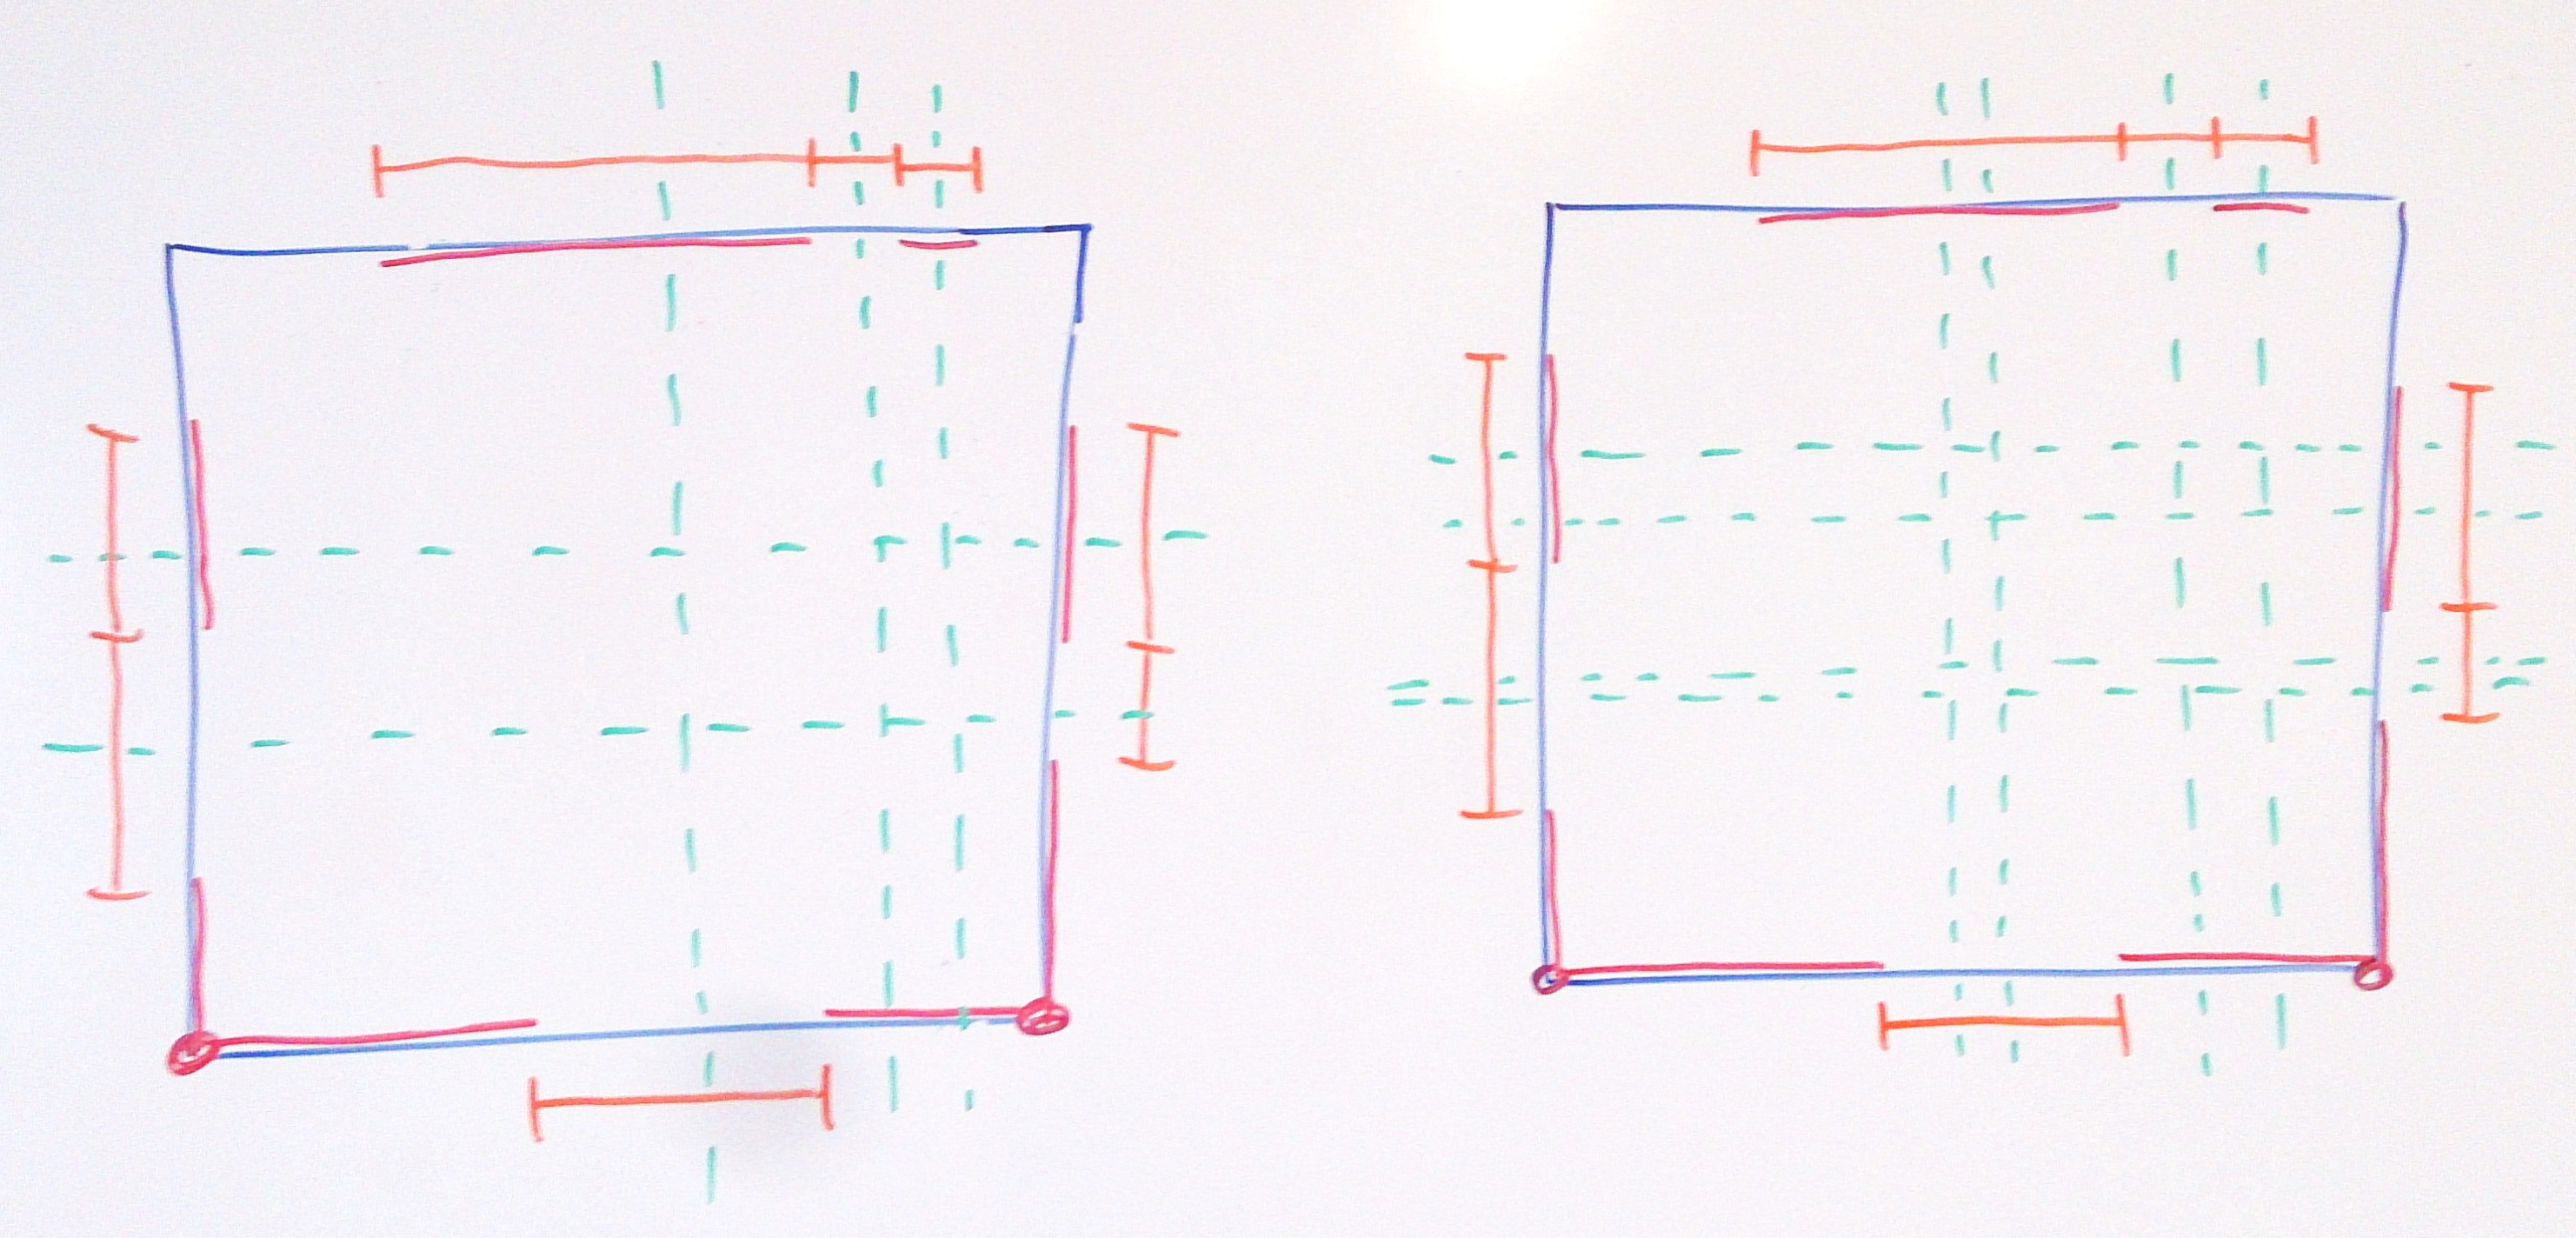
\includegraphics[width=0.9\textwidth]{images/cellslicing_dividers}
	\caption[Divider plane configurations]{
		Definition of divider planes to slice the ranges derived from the dexel segments and the space between them.
		Segments are blue, ranges in orange, dividers in dotted green lines.
		On the left drawing, dividers are set using an algorithm reducing the total number of dividers needed.
		On the right drawing, a divider is set at the midpoint of each range, resulting in more dividers but maintaining consistency with neighboring cells.
	}
	\label{fig:cellslicing_dividers}
\end{figure}

Most of the work when slicing cells is done in the \textproc{FindDiviers} function, which computes depth values for axis aligned planes along which an irregular cell should be sliced.
The function consists of two steps.
The first is to define depth ranges along each axis which have to be split.
These ranges are basically dexel segments as well as the space between two segments.
The second is to split each of this ranges by at least one divider plane.
\Cref{fig:cellslicing_dividers} illustrates these steps on a cell with calculated depth ranges in orange and two possible divider configurations in green.

The depth ranges are computed for each axis, by iterating over all twelve edges of the cell and computing the same variables as in the regularization \cref{alg:tri_dexel_regularization}, \crefrange{line:reg_vars_begin}{line:reg_vars_end}.
Using these variables, the algorithm checks if the current edge is irregular, which is the case if
\begin{itemize}
	\item both grid points are occupied and more than one segment is present,
	\item both grid points are non-occupied and any segment is present,
	\item only one of the grid points is occupied and more than one segment is present.
\end{itemize}
The segments of each irregular edge are passed to the \textproc{SegmentsToRanges} function, which determines the depth ranges which have to be sliced, and stored for the current axis.

When all depth ranges have been computed, dividers are calculated.
There are different possibilities for setting dividers.
Two variations are given in \cref{fig:cellslicing_dividers}.
The first one tries to collect as many ranges as possible which are able to be sliced by the same divider.
The second one just creates a divider at the midpoint of each range.
Whereas the first method creates fewer dividers and therefore fewer sub cells which have to be reprocessed, the second one is consistent across neighboring cells as two cells attached to the same irregular edge will create the same dividers.

In \cref{alg:tri_dexel_cell_slicing}, the first method is implemented as it produces overall better results.
Dividers are computed per axis from the list of ranges found for the current axis, sorted by the start of the ranges.
On each axis, the first divider is the bounding box itself, \ie the component of the lower vertex of the box corresponding to the current axis.
Then, an interval $(\var{start}, \var{end})$ is set to the first range, indicating a range of possible dividers.
This interval is now iteratively adapted/narrowed to span as many ranges as possible.
For this purpose, a loop iterates over all remaining ranges.
If the start of the current range does exceed the current interval, \ie the start of the range is larger than the end of the interval, a divider is created for the current interval and the interval reset to the current range.
If the current range does not exceed the current interval, \ie the start of the range lies within the interval, it is narrowed by moving its start to the start of the current range.
The end of the current interval is also adapted.
After looping over all ranges has completed, a further divider is also calculated for the remaining interval.
Finally, the upper vertex of the bounding box is used to create a last divider.
As last step, the dividers are returned and used for the creation of the bounding boxes of sub cells.

The \textproc{SegmentsToRanges} function is a simple selector and translator of dexel segments and their space between them.
The algorithm creates the ranges on each axis which must be sliced, \ie for which a divider has to be created.
In order to do so all segments of an edge are flattened into a list of start and end depth values, except values which are at the border of the cell, \ie equal to \var{srcDepth} or \var{dstDepth}.
Then, each pair of neighboring depth values are grouped into a tuple, creating a list of depth ranges.
These ranges are shown in orange in \cref{fig:cellslicing_dividers} and returned at the end of the function.


\subsection{Parallelization}
\label{sec:tri_dexel_parallelization}

The tri-dexel surface reconstruction algorithm shown in this chapter consists of a number of steps.
The first one is the creation of a tri-dexel image by raycasting the data model of the VML.
The size of the tri-dexel image and therefore the number of created rays is parameterized by the user.
Typical resolutions range from 50 for quick approximations up to several hundred\footnote{Resolutions of up to 600 were successfully tested before hitting the \SI{16}{\gibi\byte} physical RAM limit on the used machine.} for fine and detailed reconstructions.
As the number of created rays for a cubic grid with a resolution of $n$ is $3n^2$ and the ray traversal and intersection is perfectly isolated, parallelization of the raycast is embarrassingly simple and usually yields a high number of independent work items.

Concerning the implementation, all three for loops in \cref{alg:tri_dexel_raycast} are viable candidates for parallel execution.
These are the loop iterating over the three coordinate system axes as well as the loops enumerating all ray origins.
Note that the closure called for each hit, \var{hitFunc}, is invoked concurrently.
However, as the number of required dexels is derived from the user specified resolution, the tri-dexel image can preallocate all space required for the raycast result, except the list of nodes per dexel, allowing parallel access.
As a single dexel is only filled by a single ray, no concurrent access occurs on the dynamically resizing dexel lists.

The efficiency of the raycast could be furthered pushed by vectorization or GPU acceleration.
Both of these techniques have been implemented for the raycast used for visualization, \cf \cref{sec:raycasting}.
However, as the consistency of the dexel image is regarded more important than the speed of its creation, a considerable amount of additional correction code has been added to the raycast.
This code complicates vectorization and GPU acceleration, especially as the latter still does not support dynamic memory allocation on every platform\footnote{CUDA offers malloc in kernels, OpenCL has no equivalent.}.
Furthermore, the list of dexel nodes is a dynamic data structure and filled differently by each ray/thread/work item leading to even more complex vector code or branch divergence on GPUs.

When the creation of the tri-dexel image is complete, the tri-dexel grid is built by assigning all cell edges and grid point occupancies.
This task is also embarrassingly parallel at dexel level.
Considering \cref{alg:tri_dexel_grid_generation}, the outer three for loops, iterating over the three axes and then over all dexels, are almost completely independent and offer good parallelization candidates.
Assigning the segments on each dexel in parallel is also possible, but requires concurrent segment insertion at a cell edge to be safely, \cf \cref{line:grid_edge_insertion}.
If the outmost loop on the three axes is parallelized, note that the grid point occupancies are then written concurrently as the occupancy of a single grid point is determined by one dexel from each axis image.
This race condition might not be a problem on some architectures, as the same value, \True, is written concurrently to the same memory location.
However, the result depends on several hardware parameters and the memory model of the language.
For portable consistency, either the outmost loop on the axes must be serial, or the writes to the grid point occupancies atomic.

Once the tri-dexel grid is constructed, all cells have to be processed.
The required algorithms, \ie regularization, triangulation and slicing, operate independently on each cell and may therefore run in parallel.
However, the information a cell contains, \ie grid point occupancies and segments on edges, is shared between neighboring cells.
Algorithms modifying a cells data are therefore subject to race conditions.
This mainly concerns the regularization which changes the segments on cell edges.
Several solutions are available to mitigate this issue.
One possibility is locking the edge of a cell during regularization.
Neighboring cells regularized later would then see this edge as already regularized.
Unfortunately, this solution does not work well with the detection of irregular edges and cell slicing strategy, where cells are intentionally kept irregular during regularization.
Furthermore, a huge amount of locks, $\mathcal{O}(n^3)$, would be necessary, putting pressure on the operating system kernel.
A lock-free implementation of the data structure of an edge and regularization rules using atomic operations might be possible, but is probably highly difficult to achieve.
A more pragmatic solution, which has been implemented, is to just copy the data of each cell out of the tri-dexel grid before sending a cell to the regularization and subsequent algorithms.
This allows fully independent cell processing, enabling the loop on all cells in \textproc{Reconstruct} in \cref{alg:tri_dexel} to run in parallel.

The following algorithms still offer a small degree of parallelism.
However, as the independent processing of each cell already offers enough work items to saturate a large number of cores, further, nested parallelism is probably not necessary.
Nevertheless, for completeness, they are mentioned shortly.
The regularization of a cell immediately boils down to regularizing all twelve edges of the cell.
These might be regularized in parallel.
The \textproc{FindLoops} routine starting the depth-first searches on the cell might run its eight searches in parallel, accumulating the loops on a concurrent data structure.
These loops may be further triangulated in parallel in \textproc{TriangulateCell}.
Intermediate point calculation during refinement on each vertex pair of a loop might also be done in parallel, but is probably not worth the overhead.

In the underlying implementation, parallelization has been applied where suitable, again using the PPL of Microsoft and the parallel\_for primitive \cite{ppl_parallel_for}.
